\documentclass[UTF8]{ctexart}
\usepackage[utf8]{inputenc}
\usepackage{tabu}
\usepackage{geometry}
\usepackage{CJK}
\usepackage{indentfirst}
\usepackage{amsmath}
\usepackage{graphicx}
\usepackage{multirow}
\usepackage{cite}
\usepackage{tikz}

\usepackage{algorithm}
\usepackage{algorithmic}
\usepackage{float}
\usepackage{lipsum}
\usepackage{subfigure}

\CTEXsetup[format={\Large\bfseries}]{section}
\usetikzlibrary{arrows, shapes, positioning, calc, mindmap}

\makeatletter 
\renewcommand{\@thesubfigure}{\hskip\subfiglabelskip}
\makeatother

\makeatletter
\newenvironment{breakablealgorithm}
{% \begin{breakablealgorithm}
	\begin{center}
		\refstepcounter{algorithm}% New algorithm
		\hrule height.8pt depth0pt \kern2pt% \@fs@pre for \@fs@ruled
		\renewcommand{\caption}[2][\relax]{% Make a new \caption
			{\raggedright\textbf{\ALG@name~\thealgorithm} ##2\par}%
			\ifx\relax##1\relax % #1 is \relax
			\addcontentsline{loa}{algorithm}{\protect\numberline{\thealgorithm}##2}%
			\else % #1 is not \relax
			\addcontentsline{loa}{algorithm}{\protect\numberline{\thealgorithm}##1}%
			\fi
			\kern2pt\hrule\kern2pt
		}
	}{% \end{breakablealgorithm}
		\kern2pt\hrule\relax% \@fs@post for \@fs@ruled
	\end{center}
}
\makeatother

\bibliographystyle{unsrt}
\geometry{left=2.0cm,right=2.0cm,top=3cm,bottom=3cm}

\title{面向VR头盔的实时真实感绘制系统}
\author{}
\date{\today}
\begin{document}
\maketitle
\begin{abstract}
    虚拟现实(VR)是一种能为我们提供具有一定真实感的沉浸式体验的图形学技术,这一技术的快速发展对画质和渲染速度提出了越来越高的要求。
    基于OptiX光线追踪引擎,我们搭建了一个VR平台上高度真实感绘制的框架,并提出了利用GPU共享内存和VR渲染双眼图像非独立性的优化方案,
    在保证渲染效果的前提下改善了实时交互体验。
\end{abstract}

\section{介绍}
    目前VR渲染方式的主流仍然是光栅化渲染。虽然在各种技术如阴影贴图、预烘焙的光照图等方式的改善下,真实感得到了很大提高,但是仍然很难处理光照条件
    复杂的场景。光线追踪是解决这个问题的一种方案,但是其与生俱来的计算复杂度,要求必须采用蒙特卡洛方法才能达到实时的性能。而蒙特卡洛方法具有的缺
    陷是当采样数不够时,即使使用了强大的神经网络降噪模型,仍然会由于信息量不够而直接难以获得很好的效果,这一现象在实时渲染领域尤其明显。
    本文采用光子映射的方式来避免像素级别的噪点,提升观感。
    \subsection{光线追踪和光子映射}
        长期以来,快速绘制具有高质量真实感的画面一直是计算机图形学的目标。在诸多的算法中,光线追踪提供了一种成功的模拟全局光照明的方案。
        如\cite{GlobalIllumination}所述,光线追踪算法以摄像机为起点,朝着屏幕每个像素点的方向发射光线,这些光线在场景中与表面进行交
        互与传播,最终击中一个光源或发光体,并由此计算像素点的颜色。
        
        光子映射算法是光线追踪算法诸多变种中的一种。最早来源于反向光线追踪\cite{ARVO1986Backward},然后Jensen使用k最近邻估计对算法进行
        了改进\cite{Jensen1996Global}。光子映射是一种双通道方法,在第一个通道(光子追踪通道)中,光源向场景发射携带有能量(也称为通量)的光子,然后这些光子在
        场景中与表面进行交互。光子的副本会在相交的非光泽表面上被记录,并存储在被称为光子图的数据结构中。第二个通道(绘制通道)从摄像机向场景中发射光
        线,在交点处使用光子图中邻近的光子来进行亮度的估算(这个过程被称为光子密度估计)。假设点$x$附近的区域是局部平坦的,这个点
        沿$\omega$方向的辐射亮度可以用公式\ref{equ:1}来计算,其中$r$是包含了这$n$个光子的球的半径,$f_r(x,\omega_p,\omega)$是点$x$处的BRDF反射系
        数,$\Delta\Phi_p(x,\omega_p)$是第$p$个光子的能量。
        
        \begin{equation}
        L_r(x,\omega)\approx\frac{1}{\pi r^2}\sum_{p=1}^nf_r(x,\omega_p,\omega)\Delta\Phi_p(x,\omega_p)
        \label{equ:1}
        \end{equation}
    \subsection{CUDA和OptiX}
        CUDA(Compute Unified Device Architecture,统一计算架构),是由NVIDIA所推出的一种通用并行计算架构。而基于CUDA的OptiX\cite{2010OptiX}是
        一个在GPU上实现光线跟踪的应用程序框架,它提供了一个简单、递归和灵活的管道来加速射线跟踪算法。通过可编程的相交,光线生成和阴影,将NVIDIA GPU的功
        能带入光线跟踪应用程序。这两者的编程语言都是CUDA特化的C++,这种接近硬件底层的抽象程度使得用户能最大程度地利用好现有的硬件能力,包括利用GPU上的
        可以指定的共享内存,同一warp的线程同步等特性进行进行加速。NVIDIA Turing和Ampere架构显卡具有专门用于光线求交(包括与三角形求交和BVH
        遍历)的硬件电路,相比传统的在着色器里面自己实现的光线求交快数倍。而且其还保留对自定义的其他种类图元求交的支持,只要提供求交
        函数和最小包围盒的函数即可。在大多数情况下具有硬件加速的三角形求交性能会远好于其他图元,而且在现代大型游戏中基本上所有的三维网格都是由三
        角形构成的,所以这里本文中的场景将只采用三角形图元,数量为中等规模。
    \subsection{VR和OpenVR}
        VR(Virtual Reality,虚拟现实),作为一种具有强大交互能力的表现方式,已经兴起于各种需要实时交互的领域,如教育、医疗、模型设计和军事训练等等。OpenVR作
        为被多个VR设备厂家支持的API标准和SDK,作为VR硬件和软件的接口对市面上多种VR设备具有良好的兼容性。又因为其API语言也是C++,与CUDA和OptiX能完美契合,所以我们
        选择OpenVR作为给VR硬件开发的API。
    \subsection{我们的贡献}
        为了在实现光子映射的同时保证较高的实时性,我们做出了以下贡献:

        1、基于OptiX光线追踪引擎,搭建了VR头盔上高度真实感绘制的框架;

        2、提出了一种利用在VR设备中双眼图像的相关性,减少重复操作以加快绘制的方法;

        3、提出了一种利用显卡共享内存,加快光子映射算法的密度估计过程的方法;

        4、通过改善内存访问模式、利用硬件加快并行等方法加速绘制过程,在简单场景下达到了实时渲染的帧率要求。
\section{基本框架}
    本项目涉及到很多库,例如模块化的交互输入处理,传递渲染数据的OpenGL,作为异构计算的重要组成部分的CUDA,导致整个
    项目框架比较庞大,所以需要搭建一个良好的框架并使用抽象的面向对象编程来逐一完成这些任务。图\ref{fig:0}是项目框架的示意图:\\
    
    \begin{figure}[h]
        \centering
        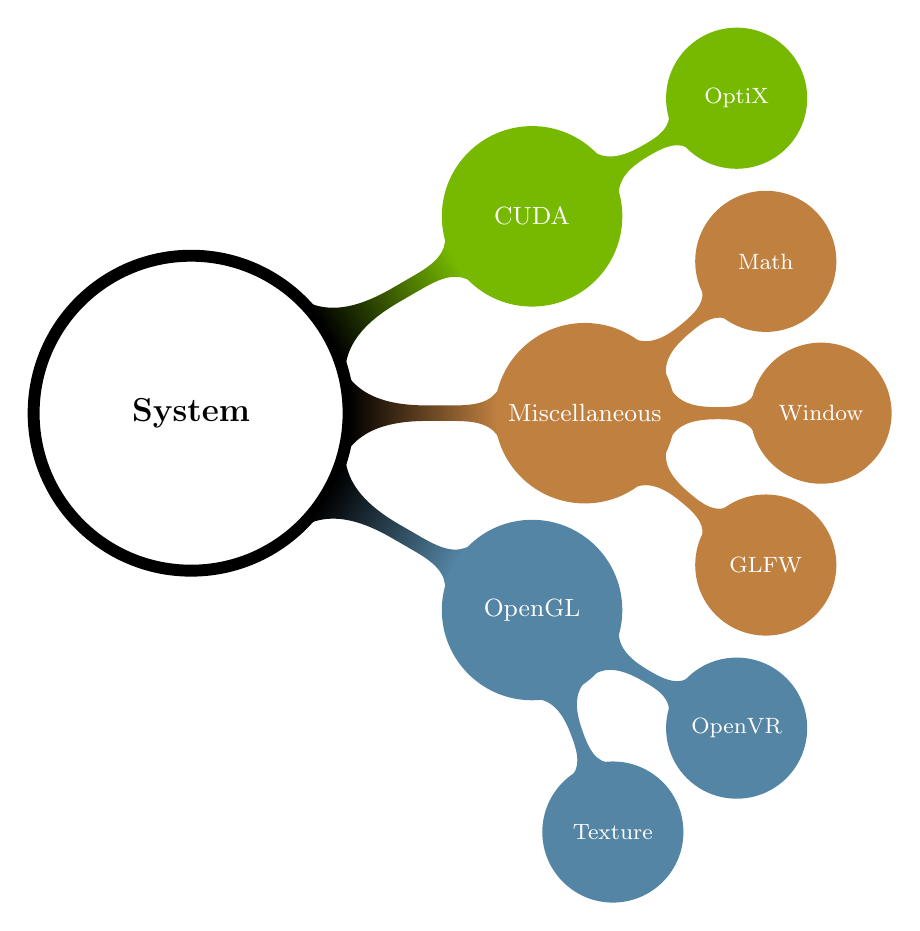
\begin{tikzpicture}
            [
                mindmap,
                every node/.style={concept, execute at begin node=\hskip0pt},
                root concept/.append style=
                {
                    concept color=black, fill=white, line width=1ex, text=black
                },
                text=white,
                grow cyclic,
                level 1/.append style = {level distance = 5cm, sibling angle=90},
                level 2/.append style = {level distance = 3cm, sibling angle=45}
            ]
            \definecolor{nvGreen}{rgb}{0.462, 0.725, 0}
            \definecolor{glBlue}{rgb}{0.33203125, 0.5234375, 0.6484375}
            \node [root concept] {\textbf{System}}
            child [concept color=nvGreen, grow=30]
            {
                node {CUDA}
                child{node {OptiX}}
            }
            child [concept color=glBlue, grow=-30]
            {
                node {OpenGL}
                child[grow=-30]{node {OpenVR}}
                child[grow=-70]{node {Texture}}
            }
            child [concept color=brown, grow=0]
            {
                node {Miscellaneous}
                child[grow=40]{node {Math}}
                child[grow=0]{node {Window}}
                child[grow=-40]{node {GLFW}}
            };
        \end{tikzpicture}
        \caption{项目框架图}
        \label{fig:0}
    \end{figure}
    \subsection{CUDA}
        CUDA框架主要是对CUDA中Buffer和纹理的封装,使得OptiX能顺利读取各种纹理和Buffer数据等。还包含了一个简化版的随机数库,用于在光追中快速生成随机数以采样。
    \subsection{OpenGL}
        OpenGL框架包含了基础的OpenGL特性的抽象封装,包括各种Buffer,对着色器的编译和渲染程序的封装等等,但是并没有类似游戏引擎的过度封装,即渲染管线仍然
        是可以高度自定义的。例如在这个光追VR项目中我们将OpenGL中的Pixel Unpack Buffer传给CUDA和OptiX渲染,完成后将其转换为Texture Buffer,再由OpenGL渲染到窗
        口和另外2个(左右眼)提交给OpenVR的纹理上,这样就算完成了一次左右眼及窗口的渲染。
    \subsection{杂项}
        剩下的杂项包含图形学常用数学库、窗口管理和GLFW库控制的交互。其中数学库包含了各种低维向量和矩阵的运算,如求矩阵逆和矩阵转置等操作。这些操作
        在处理从OpenVR得到的各种变换矩阵和位置向量的时候十分有用;窗口管理则具备了管理多个Windows窗口的能力,虽然这里只用上了一个用于同步展示头盔内部图像的
        窗口;GLFW库则是用于管理键盘鼠标控制交互的库。
\section{方法}
    \subsection{改善内存访问模式}
        传统的光子映射算法\cite{jensen2000practical}常常选用kd-树\cite{1975Multidimensional}作为保存光子图的数据结构,它会将光子平均地进行划分然后保存在数
        据结构当中。光子的位置被看做三维的向量,每个分量都被看做作为划分依据的键值。在进行划分的时候,需要首先计算一个包含所有光子的包围盒的尺寸,然后以这个
        包围盒最长边所在维度最中间的光子作为结点。这个光子在划分维度上的键值形成了一个平面,将剩余的光子平均分成两部分。这两部分光子将被分别分配到两棵子树
        当中,继续递归执行划分的过程,直到不能继续划分为止。为了避免使用指针的开销,在实际实现中可以使用完全二叉树数组来表示kd-树。
        
        在密度估计时需要搜索某个点附近的光子,整个搜索过程从kd-树的根结点开始,计算这个点和根结点光子之间的距离,如果小于设定的半径,那么就要计算根结点光子
        对结果的贡献。然后计算这个点相对于根结点的位置,和这个点同一侧的光子都是可能对最终结果有贡献的,在这部分光子对应的子树上递归调用搜索过程。如果这个
        点到根结点光子所产生的划分平面的距离小于设定的半径,那么另一侧的光子也有可能对最终结果产生贡献,也需要对另一侧光子对应的子树递归调用搜索过程;否则
        另一侧的光子和这个点的距离都一定大于设定的半径,不会产生贡献,可以直接抛弃。
        
        使用kd-树可以避免对所有光子的搜索,从而提高了搜索的效率。但是这种数据结构的问题是访问的随机性太高,在搜索过程中先后进行搜索的两个光子在内存中的位置
        并没有什么相关性,甚至可能隔得很远,这样就没有办法充分利用硬件设备的带宽。在光子映射算法中,最近光子搜索占据了主要的开销\cite{gupte2011real},如果
        不能充分利用带宽,那么这个部分就会成为整个算法的瓶颈。
        
        我们将光子图的数据结构改换为哈希网格\cite{fleisz2009photon},它的主要思想是这样的:将空间均匀划分为大量的小立方体,定义的哈希函数将位于小立方体内的
        坐标映射成这个小立方体的编号,同一个小立方体内的光子在内存中相邻保存,这样搜索某个点附近的光子时,只需要搜索可能有贡献的小立方体对应的一片片连续的内
        存空间即可。
        
        为此我们需要首先计算整个网格的大小,网格的原点被设定成各个分量都最小的光子的坐标gridOrigin(可以比这个坐标再小一点)。方便起见,每个小立方体的边长
        被设定为搜索半径的大小r,这样在搜索的时候每个点在搜索的时候只需要访问以它所在的小立方体为中心的$3\times3\times3$的区域即可。将整个网格的大小除以每
        个小立方体的边长并向上取整,可以获得网格各个维度的小立方体数量,记为gridSize。我们采用了\cite{gupte2011real}中的做法,在每个维度的两端额外添加一层
        小立方体,用增大内存开销的方式避免了边界检查。哈希函数采用了简单易实现的线性映射:
        \begin{equation}
        hash(photon)=z \times gridSize.x \times gridSize.y + y \times gridSize.x + x
        \label{equ:2}
        \end{equation}
        
        其中$x=\lfloor(photon.x-gridOrigin.x)/r\rfloor$,是光子相对于网格原点的位置除以小立方体边长向下取整的结果,$y$和$z$的计算与$x$类似。
        
        获取了哈希函数的计算式之后,可以计算原始光子图中的每个光子的哈希值(也就是所在的小立方体的编号),然后根据哈希值从小到大的顺序将光子重新排序,这样就
        完成了光子图的构建。除此之外,还需要生成一个前缀和数组startIdx,记录每个小立方体所包含的光子的起始下标,编号为i的小立方体所包含的光子从
        下标startIdx[i]开始,一共startIdx[i+1]$-$startIdx[i]个。包括中心小立方体在内的27个小立方体的编号相对于中心小立方体的编号的偏移都是固定的,可以事
        先计算好,然后保存在一个偏移查看表中,在搜索的过程中查表就可以知道下一个待搜索的小立方体的编号的偏移。更高效的做法是利用相邻编号的小立方体的光子是紧
        挨着保存的特点,只在偏移查看表中储存9个条目。
        
        重构光子图的过程如图\ref{fig:1}所示:左上图是场景中光子分布的示意,其中小立方体的编号用红色表示,光子的编号用黑色表示。右上图计算了场景中的每个光子
        的哈希值,在此之后依据哈希值从大到小将光子重新排序,下图是扫描得到的前缀和数组startIdx,它表明在0、7、9、14号小立方体中分别存在1、1、2、1个光子。
        
        \begin{figure}[H]
            \centering
            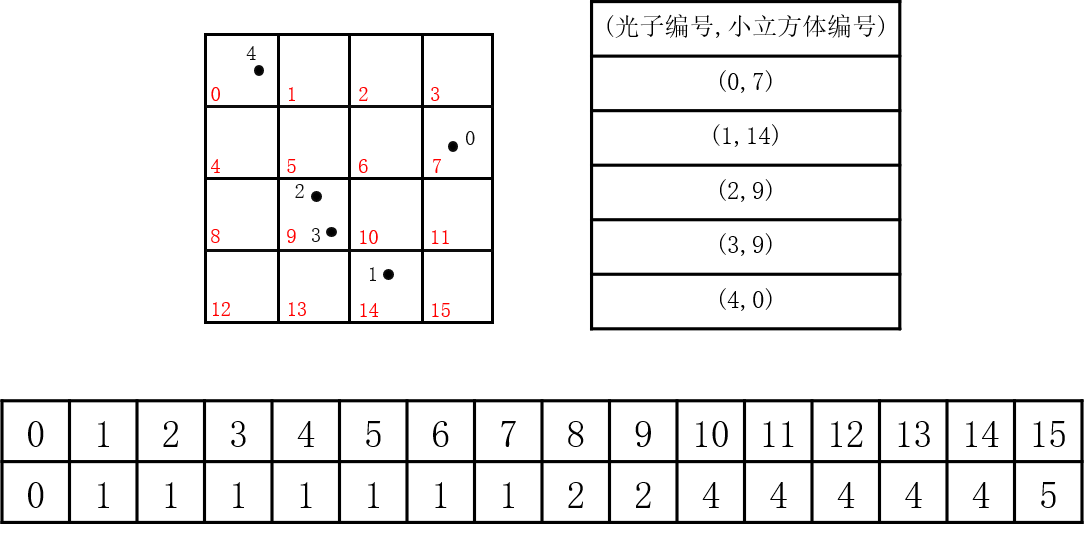
\includegraphics[scale=0.6]{pic/HashGridPhotonRebuild.png}
            \caption{哈希网格光子图重构示意图}
            \label{fig:1}
        \end{figure}
        
        在哈希网格中进行搜索的过程如图\ref{fig:2}所示,蓝点代表需要进行密度估计的点,它所在的小立方体的编号为10,根据偏移查看表,光子图中下标从startIdx[5]开始
        到startIdx[8]之前,从startIdx[9]开始到startIdx[12]之前,从startIdx[13]开始到startIdx[16]之前的光子可能会对这个点产生贡献,也就是0,2,3,1号光子。最终0号
        光子由于距离过远被剔除,其他的光子参与最终贡献的计算。
        
        \begin{figure}[H]
        \centering
        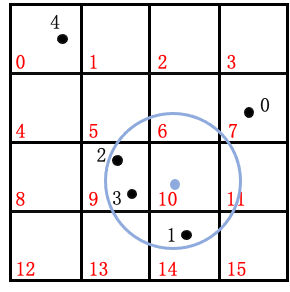
\includegraphics[scale=0.6]{pic/HashGridSearch.png}
        \caption{哈希网格搜索}
        \label{fig:2}
        \end{figure}
        
        当kd-树和哈希网格所需要搜索的光子数差不多的时候,由于哈希网格访问的内存地址更加紧凑有序,这种方法将更加有效。这一方法存在的缺陷是,为了不漏掉搜索半径内
        的任何光子,必须完整搜索周围的27个小立方体,这就可能有大量不会产生贡献的光子被访问到。最糟糕的情况下,光子均匀分布在网格中,只有$\frac{4}{3}\pi\div27\approx15.5\%$被访问
        的光子产生贡献,这个情况是使用kd树时不会发生的。幸运的是,很多情况下这一效率并没有这么低,这部分效率的损失被紧凑的内存访问所弥补,最终表现出比kd-树更好的性能。
        
        与kd-树相比,使用哈希网格需要额外的一个前缀和数组的空间开销。而且由于空间的均匀划分和场景的非均匀分布,小立方体内包含的光子数目差别很大,许多小立方体内部都是空的。
        
        光子映射算法在进行密度估计时,一般使用k最近邻算法(k-nearest neighbors,kNN),它需要获取给定位置附近的k个最近的光子。kNN算法需要为此维护一个大小为k的最大堆
        \cite{jensen2000practical},使用最大堆可以很方便地追踪堆中光子距离估计点距离的最大值,如果当前堆中光子个数不到k,那么可以直接将访问到的新光子插入堆中,如果堆中已经
        包含了k个光子,并且新访问到的光子比堆中距离最远的光子更近,那么可以删除堆中最远的光子,然后将新访问到的光子插入。在最大堆被填满之后的搜索过程中,可以使用位于根结点的光子的距离
        作为限定,大于此距离的光子将全部被舍弃。在堆中最远的距离将作为算法\ref{equ:1}估计时的半径。正是由于前面所说到的这个“半径收缩”的过程,最后用于密度估计的半径会比
        事先给定的半径小\cite{2003Photon}。
        
        图\ref{fig:6}(左)展示了在使用kd-树作为光子图数据结构时实施kNN算法的过程,选取$k=3$,图中的黑色点代表光子,蓝色点代表给定的需要进行密度
        估计的点,黑色点虚线代表kd-树进行划分的平面,为了清楚起见,叶子结点的划分平面被略去了,蓝色虚线圈代表事先给定的半径范围,而蓝色实线圈代表最后用于密度估计的半径范围。
        最大堆会首先被蓝色实线圈内的三个光子所填满,然后发生了“半径收缩”,位于蓝色实线圈和蓝色虚线圈之间的光子距离远于此时的半径,所以被排除在外,另外的三个光子由于距离过大也被排除。

        图\ref{fig:6}(中)则展示了使用哈希网格作为光子图数据结构时实施kNN算法的过程,最大堆会先被与给定点位于同一个格子内的三个光子填充,然后在访问位于右下角的光子的时候,发现距离比
        当前堆中最远的光子(蓝色实线圈与蓝色虚线圈之间的光子)要近,于是进行替代并发生了“半径收缩”。值得一提的是,利用图\ref{fig:6}可以展示哈希网格的缺点:在使用kd-树的方案中,
        虚线圈外的三个光子由于给定点到它们的分隔平面距离过远,都是不需要访问的,而在使用哈希网格的方案中,由于所有的光子都在给定点周围的方格内,所有的光子都需要被访问到。

        \begin{figure}[H]
        \centering
        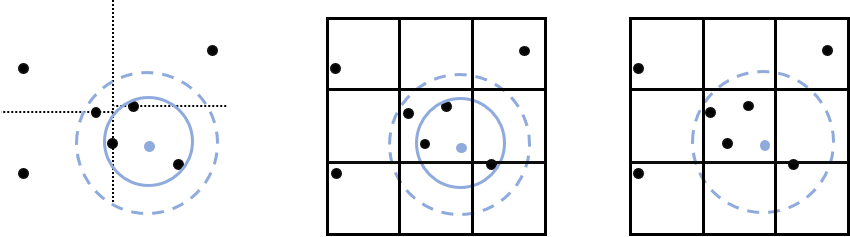
\includegraphics[scale=0.8]{pic/KNN.png}
        \caption{堆与KNN示意图}
        \label{fig:6}
        \end{figure}

        在具体的实现中,较小的堆会导致生成明显的图像偏差,而较大的堆则则不得不被分配到显卡的全局内存中,大量的全
        局内存访问和维护堆的操作开销将阻碍实时渲染的实现。为此,我们选择不使用堆,计算搜索半径内所有光子的贡献。
        如图\ref{fig:6}(右)所示,这样做会使最终的估计半径会比使用堆时的估计半径大,这样的后果是:一方面,最靠近带搜索点的光子(蓝色实线圈内的光子)的贡献会相应降低,
        另一方面,更多的光子(蓝色实线圈和蓝色虚线圈之间的光子)会参与贡献的计算。

    \subsection{利用硬件能力加速}
        虽然OptiX是个高效的光线追踪引擎,但是由于其实现是基于不同像素光线不存在相关性的假设,所以如果使用了多线程协作,OptiX则无法进行处理。为此,我们编写了两种内核
        函数并进行了对比:一种采用纯OptiX内核执行光线追踪和光子密度估计,另一种使用OptiX进行光线追踪,而采用CUDA进行光子密度估计。
        
        通常,光子图存储在显卡的全局内存当中。负责执行任务的流多处理器可以使用位于芯片之上的共享内存,这部分内存的访问比全局内存更快,而且更重要的一点是,共享内存中的数据
        可以被一组线程共享。为了充分利用共享内存,提高带宽利用率,我们设计了如下方案:
        
        首先,整个屏幕被划分成一些粗粒度的网格,每一个格子被分配给一个CUDA线程组,格子内的像素的计算任务被分配到单独的线程。首先由每一个线程计算当前像素对应的光线与场景的
        交点所处的哈希小立方体的编号,如果线程组内所有线程得到的编号都相同,说明网格内的所有像素光线都最终交于同一个哈希小立方体,它们将对完全相同的$3\times3\times3$区域内
        的光子进行遍历。现在,每个线程从所需要遍历的光子中选取一部分,将它们从全局内存中读入到共享内存当中,然后每个线程对共享内存内的光子再进行遍历。图\ref{fig:5}(右)是
        对这一过程的说明,最上方的两个小圆代表计算像素颜色的两个线程,假设它们一共需要访问全局内存中储存的4个光子,那么它们首先会将全局内存中的两个光子加载到共享内存中,每
        个线程加载一个光子(由黑色实线箭头表示),然后这两个线程会从共享内存中获取光子的信息,然后进行密度估计(黑色点虚线箭头表示)。然后这两个线程再次从全局内存中加载另外
        的两个光子到共享内存(蓝色实线箭头表示),然后再从共享内存中读取光子信息(黑色点虚线箭头表示)。
        
        \begin{figure}[H]
        \centering
        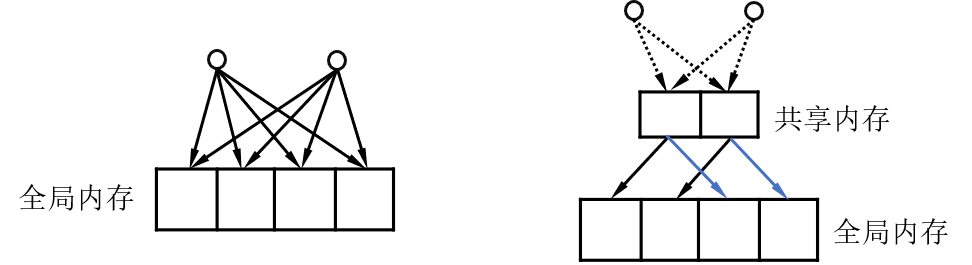
\includegraphics[scale=0.7]{pic/SharedMemory.png}
        \caption{共享内存利用示意图}
        \label{fig:5}
        \end{figure}
        
        不使用共享内存的做法图\ref{fig:5}(左)一共需要进行$2\times4=8$次全局内存的访问,而使用共享内存的做法图\ref{fig:5}(右)需要进行$2\times4=8$次共享内存的访问和$4$次
        全局内存的访问。由于共享内存比全局内存快的多,而且现在只需要数量更少的全局内存访问,可以更加有效利用带宽来加快速度。算法\ref{alg:1}给出了算法伪代码:
        
        \renewcommand{\algorithmicrequire}{\textbf{Input:}} 
        \renewcommand{\algorithmicensure}{\textbf{Output:}}
        
        \begin{breakablealgorithm}
        \caption{利用共享内存进行密度估计算法伪代码}
        \label{alg:1}
        \begin{algorithmic}[1]
            \REQUIRE array offset, array startIdx, array photonMap
            \STATE photons := \textbf{shared memory}[\textbf{group size}];  /* 光子 */
            \STATE hashValues := \textbf{shared memory}[\textbf{group size}];   /* 每个交点的哈希值 */
            \STATE flag := \textbf{shared variable};    /* 是否启用算法的标志位 */
            \STATE flag := 0;
            \STATE hashValues[\textbf{group index}] := hash(hitPointPosition); /* 计算交点小立方体编号 */
            \STATE \textbf{group barrier};
            \IF{(hashValues[\textbf{group index}] != hashValues[(\textbf{group index}+1)\%\textbf{group size}]}
                \STATE flag := 1;
            \ENDIF
            \STATE \textbf{group barrier};
            \IF{flag == 1}
                \STATE 直接进行密度估计; /* 至少有一个线程的交点与其他线程不同 */
            \ELSE
            \STATE /* 所有线程交点落在同一个小立方体内 */
                \FOR{i := 0; i \textless\  27; i += 1}
                    \STATE collectedCnt := 0;   /* 当前线程已经访问的光子数 */
                    \STATE start := startIdx[hashValues[\textbf{group index}] + offset[i]];
                    \STATE end := startIdx[hashValues[\textbf{group index}] + offset[i] + 1];
                    \STATE photonCnt := end - start;/* 当前小立方体内光子数量 */
                    \STATE paddedCnt := 将photonCnt对齐到\textbf{group size}
                    \FOR{j := \textbf{group index}; j \textless\  paddedCnt; j += \textbf{group size}}
                        \IF{j \textless\  photonCnt}
                            \STATE photons[\textbf{group index}] := photonMap[start + j];
                        \ENDIF
                    \ENDFOR
                    \STATE \textbf{group barrier};
                    \FOR{k := 0; k \textless\  \textbf{group size} and collectedCnt \textless\  photonCnt; k += 1, collectedCnt += 1}
                    \STATE 读取photons[k]计算贡献;
                    \ENDFOR
                    \STATE \textbf{group barrier};
                \ENDFOR
            \ENDIF
            \STATE \textbf{group barrier};
        \end{algorithmic}
        \end{breakablealgorithm}
        
        伪代码第20行的对齐操作是很有必要的,不进行对齐的话,部分像素会少进行一次光子贡献的计算。
        值得一提的是,如果线程组中的某个线程对应的光线没有与场景相交,它也可以协助进行从全局内存到共享内存的光子加载。
    \subsection{利用双眼图像相关性加速}
        现实世界中,我们人的双眼看到的图像是不一样的,因此如果VR设备想要提供真实感,就要对双眼所看到的图像进行分别绘制。一个简易的想法是,根据VR设备传入的眼睛的
        位置和投影矩阵,分别对左右眼进行图像的渲染和显示。但是事实上,左右眼看到的图像并不是独立的,有很大一部分区域是重合的。
        
        参考文献\cite{fujita2014foveated}当中采用的做法是绘制一张比目标图像更宽的图像,然后将左边的一部分图像绘制到左眼,将右边的一部分绘制到右眼。这样做是不正确的,即使
        是看同一个物体,左右眼的方向也不完全相同,这一现象称为“视差”,它决定了双眼看到的图像在平移后不能重合。“视差”是人感受深度的重要因素之一,忽略它将导致真实感的损失。
        
        考虑到左右眼的光线可能会交于场景中的同一个点,那么这个点所对应的直接和间接光照计算就没有必要进行两次,可以将左眼的计算结果保存起来,在绘制右眼图像的时候直接读取对
        应的值即可。在简单的朗伯面漫反射情况下,BRDF函数与出射光线的方向无关,所以右眼的光强和左眼的是一致的,可以直接使用,但是若BRDF函数与出射光线的方向有关,那么还
        需要进一步的处理。
        
        我们的方法是这样的:在绘制左眼图像的时候,连接左眼和每一个左眼屏幕上的像素,产生左眼光线,判断每一个左眼光线和场景的交点对右眼的可见性,如果这个
        交点是右眼可见的,计算这个交点在右眼屏幕上的对应的像素,然后保存在该像素对应的缓存中。在绘制右眼图像的时候,检查当前像素对应的内存是否已经被绘制过了,如果已经被绘制
        过了,那就可以直接从该缓存中读取颜色;否则进行直接和间接光照的计算。
        
        整个过程如图\ref{fig:3}所示,为了计算左眼屏幕坐标为index的像素的颜色,一条左眼光线(蓝色实线)被发射到场景中,以它与场景的交点为出发点,朝右眼发射一条光线(红色虚
        线),做可见性判断,如果是可见的,就计算这个右眼光线对应的屏幕上的像素的坐标c\_index。如果这个坐标位于屏幕像素的范围内,那么在buffer[c\_index]中将记录该点在右眼
        中的颜色。这样当在绘制右眼屏幕坐标为c\_index的像素的时候,查看buffer[c\_index]发现已经有值了,于是直接将这个值读到帧缓存对应的位置中。
        
        \begin{figure}[H]
        \centering
        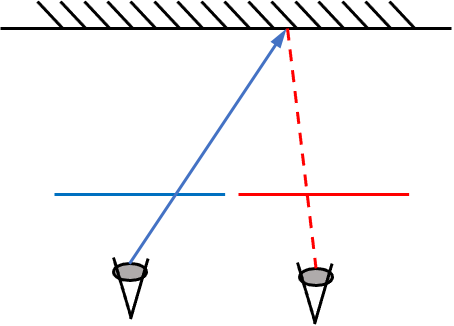
\includegraphics[scale=0.6]{pic/BinocularCorrelation.png}
        \caption{双眼图像相关性示意图}
        \label{fig:3}
        \end{figure}
        
        c\_index的计算方法是这样的:VR系统会根据输入的裁剪参数$zNear, zFar$提供一个透视投影矩阵$M_{proj}$,还会根据头盔朝向提供从世界参考系到头盔参考系的旋转变换矩阵$M_{rotate}$,头盔位置和双眼
        相对于头盔的位置(头盔坐标系)。根据这些数据可以计算出从头盔参考系到世界参考系的旋转变换矩阵$M^{-1}_{rotate}$,双眼在世界坐标系中的
        坐标$\overrightarrow{r}_{left}, \overrightarrow{r}_{right}$。用$\overrightarrow{r}_{hit}$表示世界坐标系下交点的位置,$\overrightarrow{r}_{eye}$表示世界坐标系下点相对于眼睛的
        位置,因此可以计算出在头盔坐标系中右眼观察的方向$\overrightarrow{r}_{dir}$(未归一化):
        \begin{equation}
            \overrightarrow{r}_{dir}=M_{rotate}(\overrightarrow{r}_{hit}-\overrightarrow{r}_{right})
        \end{equation}
        根据这个方向,利用投影矩阵即可得到裁剪空间的$x,y$值(范围是[-1, 1],而且由于只需要$x, y$值,所以$\overrightarrow{r}_{dir}$也可以不归一化)。设裁剪坐标是$\overrightarrow{r}_{scissor}$
        \begin{equation}
            \overrightarrow{r}_{scissor}=M_{proj}\overrightarrow{r}_{dir}
        \end{equation}
        最后裁剪坐标归一化后乘以屏幕长宽即可得到像素位置
        \begin{equation}
            \begin{array}{c}
                index.x=\lfloor\frac{1}{2}(\overrightarrow{r}_{scissor}.x+1)\times size.x\rfloor\\
                index.y=\lfloor\frac{1}{2}(\overrightarrow{r}_{scissor}.y+1)\times size.y\rfloor\\
            \end{array}
        \end{equation}
        
        由于不同左眼像素对应的右眼像素可能是同一个,所以需要一个原子操作来保证对于每个右眼像素都只被写入了一次。这时候,可以利用帧缓存中没有被利用到的$w$分量,利用atomicCAS函数
        读取并将其与某特定非零值进行比较,若相等,则表明这个像素已经被其他左眼像素对应的线程写入了,无需再写入一遍;若不相等(即为0),则表明尚未被写入,可以直接将其写入那个特定
        非零值并向$xyz$分量写入颜色信息。对计算得到的像素位置,必须进行越界检查,确保只有在屏幕范围内的像素被绘制,否则可能会造成内存访问的错误。
        
        \begin{figure}[H]
        \centering
        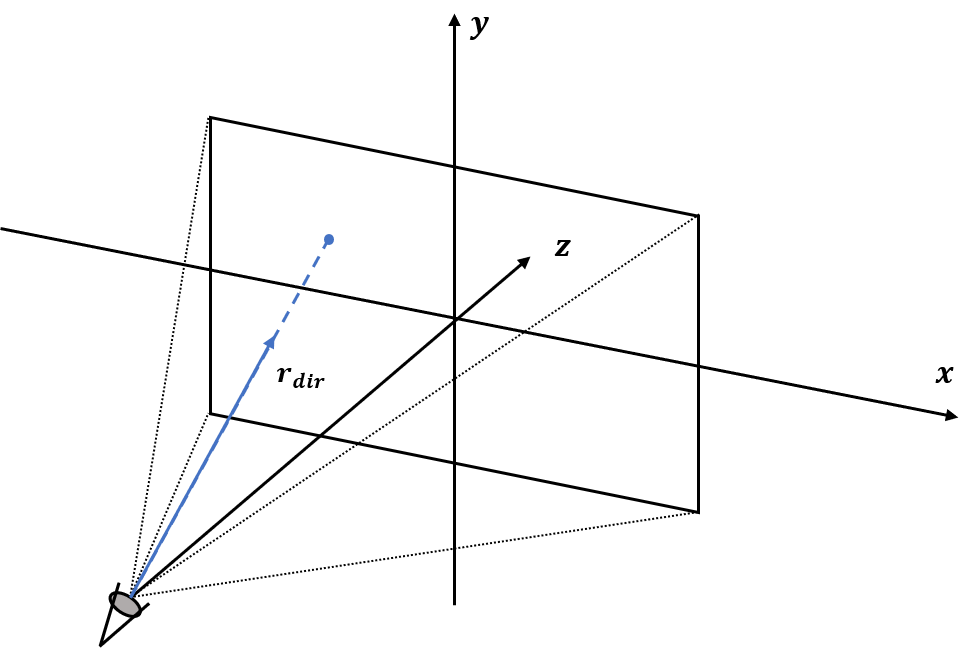
\includegraphics[scale=0.6]{pic/IndexCalculation.png}
        \caption{像素位置计算示意图}
        \label{fig:4}
        \end{figure}
\section{实验}
    \subsection{实验设备}
        我们使用的显卡是RTX2080Ti,VR设备是HTC Vive。测试得到的帧时间都是连续绘制100帧然后取平均值,前4项实验中并没有使用到VR,都是记录了单张图像的平均绘制时间,
        最后一项实验中使用了VR,记录了双眼图像的平均绘制时间。我们测试了使用不同的发射光子数和搜索半径的结果。每一项中得到的最好的结果用粗体强调。
    \subsection{实验结果}
        我们首先比较了使用传统的kd-树和哈希网格作为光子图的数据结构时的绘制帧时间,结果列在表\ref{table:1}中。可以看到,当发射的光子数和搜索半径不太大时,使用哈希网格会起
        到加速效果;当发射的光子数增多,半径也相应变大的时候。哈希网格的速度又比使用kd-树更慢了,如前文所述,哈希网格提供更紧凑的内存访问的代价是很多没有贡献的光子也会被
        访问到。在随后的实验中,我们都将使用哈希网格作为光子图数据结构。
        
        \begin{table}[H]
            \centering
            \caption{采用不同数据结构绘制帧时间的比较}
            \label{table:1}
            \begin{tabular}{ll|ll|ll}
            \hline\hline
            \multicolumn{2}{c}{参数} & \multicolumn{2}{c}{Cornell Box} & \multicolumn{2}{c}{Office}  \\
            \hline
            发射光子数 & 搜索半径 & kd-树  & 哈希网格  & kd-树  & 哈希网格 \\
            \hline\hline
            \multirow{3}*{$512\times512$} & 0.02   & 7.28ms   & \textbf{3.89ms} &    &    \\
            ~   & 0.05  & 118.35ms  & \textbf{90.74ms} &    &    \\
            ~   & 0.1   & \textbf{426.39ms}  & 501.79ms &    &    \\
            \hline
            \multirow{3}*{$256\times256$} & 0.05   & 8.32ms   & \textbf{5.23ms} &    &    \\
            ~   & 0.1  & 72.05ms  & \textbf{49.29ms} &    &    \\
            ~   & 0.2   & \textbf{287.87ms}  & 362.10ms &    &    \\
            \hline
            \multirow{3}*{$128\times128$} & 0.05   & 2.57ms   & \textbf{1.94ms}  &    &    \\
            ~   & 0.1   & 5.69ms   & \textbf{3.67ms} &    &    \\
            ~   & 0.2   & 36.29ms   & \textbf{22.90ms} &    &    \\
            \hline\hline
            \end{tabular}
        \end{table}
        
        然后我们比较了是否使用最大堆对绘制时间的影响,结果列在表\ref{table:2}中。可以看到,这一步带来的加速是显著的,背后的原因主要是减少了位于全局内存中的堆的访问以及堆
        维护的操作开销。如前所述,这样做让那些本来最终保存在堆中的光子的贡献降低,同时会计算更多本来不会被保存在堆中的光子,这样做会使得最终得到的图像更加模糊。
        
        在图\ref{fig:8}中我们展示了是否使用堆对于渲染效果的影响,左图是使用大小为128的堆得到的结果,右图是不使用堆得到的结果,两者发射的光子数都是$512\times512$,
        搜索半径都是$0.08$,除了亮度,两者的区别并不是很明显,左图比较暗的原因是128的堆大小过小,而右图可以取用数量更多的光子进行密度估计。
        在后续的实验中都不使用堆。
        
        \begin{table}[H]
            \centering
            \caption{是否使用堆绘制帧时间的比较}
            \label{table:2}
            \begin{tabular}{ll|ll|ll}
            \hline\hline
            \multicolumn{2}{c}{参数} & \multicolumn{2}{c}{Cornell Box} & \multicolumn{2}{c}{Office}  \\
            \hline
            发射光子数 & 搜索半径 & 使用堆  & 不使用堆 & 使用堆  & 不使用堆 \\
            \hline\hline
            \multirow{3}*{$512\times512$} & 0.02   & 3.89ms  & \textbf{2.33ms} &    &    \\
            ~   & 0.05  & 90.74ms  & \textbf{4.36ms} &    &    \\
            ~   & 0.1   & 501.79ms  & \textbf{11.43ms} &    &    \\
            \hline
            \multirow{3}*{$256\times256$} & 0.05   & 5.23ms  & \textbf{2.30ms} &    &    \\
            ~   & 0.1   & 49.29ms  & \textbf{3.94ms} &    &    \\
            ~   & 0.2   & 362.10ms  & \textbf{11.24ms} &    &    \\
            \hline\hline
            \end{tabular}
        \end{table}

        \begin{figure}[H]
            \centering
            \begin{minipage}[t]{0.48\textwidth}
            \centering
            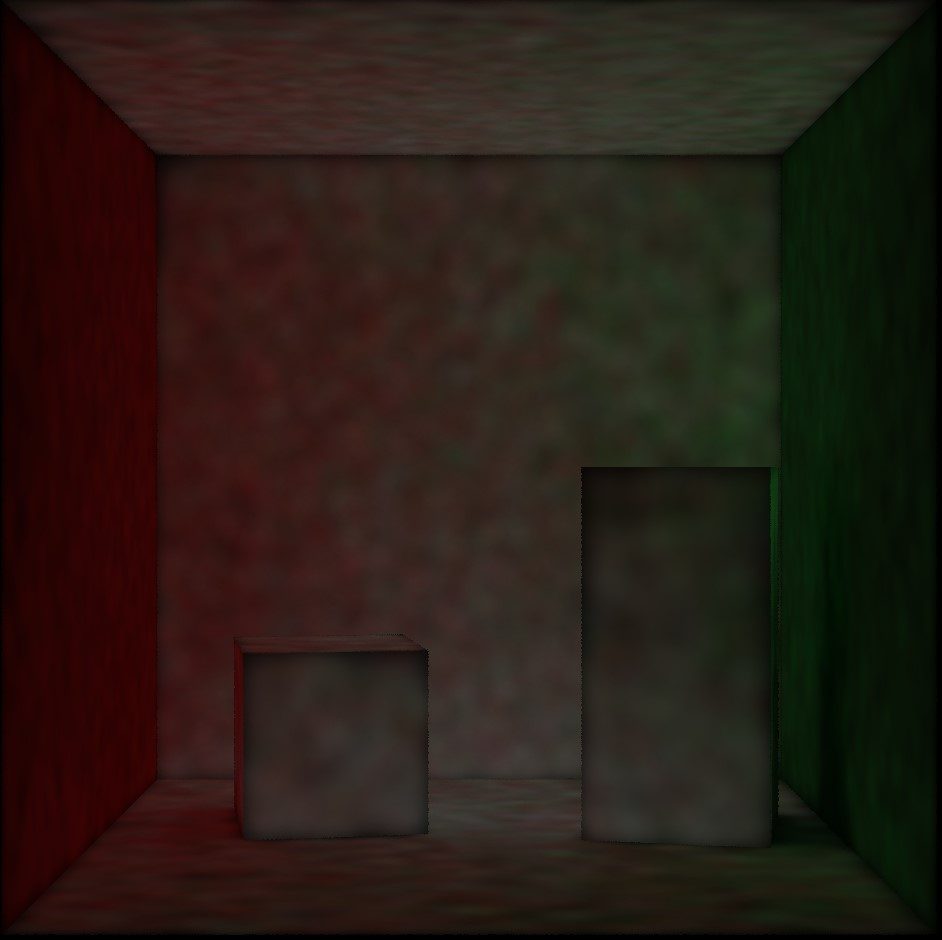
\includegraphics[width=8cm]{pic/useheap.png}
            \end{minipage}
            \begin{minipage}[t]{0.48\textwidth}
            \centering
            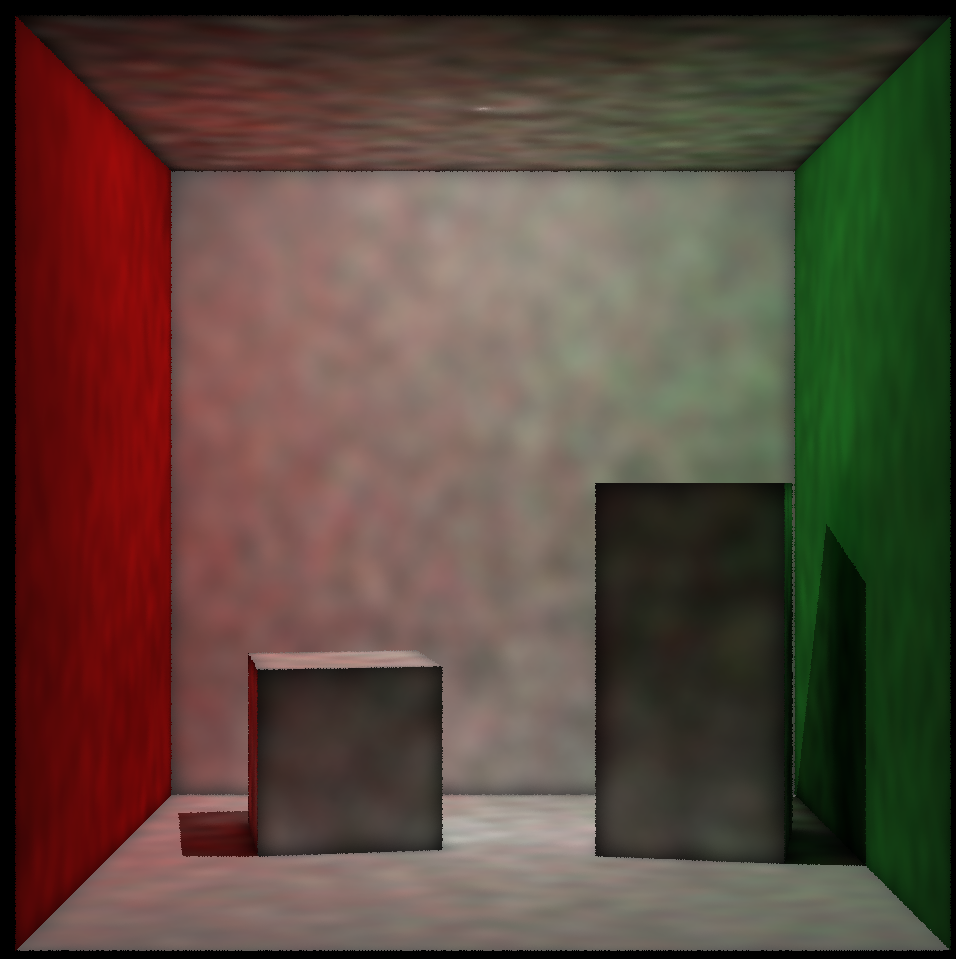
\includegraphics[width=8cm]{pic/withoutHeap.png}
            \end{minipage}
            \caption{是否使用堆的渲染效果对比}
            \label{fig:8}
        \end{figure}
        
        在表\ref{table:3}中,我们比较了使用OptiX内核同时执行光线追踪和密度估计的方案(单一方案)与只使用OptiX内核进行光线追踪而使用CUDA内核执行密度估计的方案(混合方案)。
        可以看到,即使额外增加了OptiX内核和CUDA内核之间传递交点信息的通信开销,使用混合方案大体上也只需要单一方案的一半的时间。可能的解释是,OptiX没有充分利用到CUDA的能力,
        在执行像密度估计这样更加通用的并行任务上的效率不如基础的CUDA高。在后续的实验中我们都将使用混合的方案。
        
        \begin{table}[H]
            \centering
            \caption{使用不同内核绘制帧时间的比较}
            \label{table:3}
            \begin{tabular}{ll|ll|ll}
            \hline\hline
            \multicolumn{2}{c}{参数} & \multicolumn{2}{c}{Cornell Box} & \multicolumn{2}{c}{Office}  \\
            \hline
            发射光子数 & 搜索半径 & 单一方案 & 混合方案 & 单一方案 & 混合方案 \\
            \hline\hline
            \multirow{3}*{$512\times512$} & 0.05  & 4.59ms  & \textbf{3.41ms} &    &  \\
            ~   & 0.1   & 12.39ms  & \textbf{6.52ms} &    &  \\
            ~   & 0.2   & 37.60ms  & \textbf{17.51ms} &    &  \\
            \hline
            \multirow{3}*{$256\times256$} & 0.05   & 2.60ms  & \textbf{2.31ms} &    &  \\
            ~   & 0.1   & 4.03ms  & \textbf{3.76ms} &    &  \\
            ~   & 0.2   & 10.66ms  & \textbf{6.00ms} &    &  \\
            \hline\hline
            \end{tabular}
        \end{table}
        
        在表\ref{table:4}中展示了使用算法\ref{alg:1}的效果,起到的效果并不明显,查看profile发现整个程序运行的瓶颈并不在于内存访问,而在于密度估计中用到的大量的运算。尽管
        如此,算法\ref{alg:1}提供了利用共享内存对整个密度估计进行加速的独创思路。
        
        \begin{table}[H]
            \centering
            \caption{是否使用共享内存绘制帧时间的比较}
            \label{table:4}
            \begin{tabular}{ll|ll|ll}
            \hline\hline
            \multicolumn{2}{c}{参数} & \multicolumn{2}{c}{Cornell Box} & \multicolumn{2}{c}{Office}  \\
            \hline
            发射光子数 & 搜索半径 & 不使用共享内存  & 使用共享内存 & 不使用共享内存  & 使用共享内存 \\
            \hline\hline
            \multirow{3}*{$512\times512$} & 0.05   & 3.41ms  & \textbf{3.18ms} &    &  \\
            ~   & 0.1   & 6.52ms  & \textbf{6.33ms} &    &  \\
            ~   & 0.2   & 17.51ms  & \textbf{15.88ms} &    &  \\
            \hline
            \multirow{3}*{$256\times256$} & 0.05   & 2.31ms  & \textbf{2.25ms} &    &  \\
            ~   & 0.1   & 3.76ms  & \textbf{3.06ms} &    &  \\
            ~   & 0.2   & 6.00ms  & \textbf{5.80ms} &    &  \\
            \hline\hline
            \end{tabular}
        \end{table}
        
        \begin{table}[H]
            \centering
            \caption{两种绘制方式绘制帧时间的比较}
            \begin{tabular}{ll|ll|ll}
            \hline\hline
            \multicolumn{2}{c}{参数} & \multicolumn{2}{c}{Cornell Box} & \multicolumn{2}{c}{Office}  \\
            \hline
            发射光子数 & 搜索半径 & 双眼分开绘制  & 利用双眼相关性绘制 & 双眼分开绘制  & 利用双眼相关性绘制 \\
            \hline\hline
            \multirow{3}*{$512\times512$} & 0.05   &   &   &   &   \\ 
            ~   & 0.1   &   &   &   &   \\ 
            ~   & 0.2   &   &   &   &   \\ 
            \hline
            \multirow{3}*{$256\times256$} & 0.05   &   &   &   &   \\ 
            ~   & 0.1   &   &   &   &   \\ 
            ~   & 0.2   &   &   &   &   \\ 
            \hline\hline
            \end{tabular}
        \end{table}
        在图\ref{fig:9}和图\ref{fig:10}中展示了最后的渲染效果,在Cornell Box场景中我们采用的发射光子数为$512\times512$,搜集半径为$0.2$,所需要的渲染时间为18.38ms。
        在Office场景(71万个三角片元)中我们采用的发射光子数为$512\times512$,搜集半径为$0.15$,所需要的渲染时间为11.96ms。

        \begin{figure}[H]
            \centering
            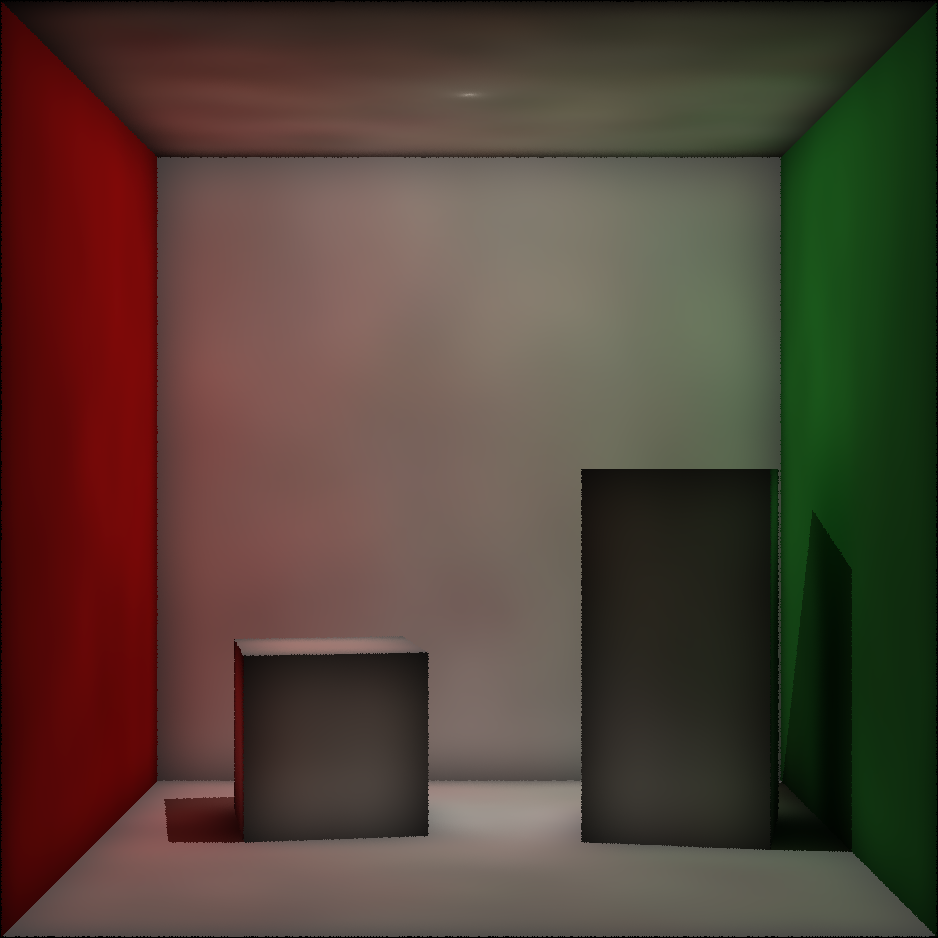
\includegraphics[width=10cm]{pic/CornellBox.png}
            \caption{Cornell Box最终渲染效果}
            \label{fig:9}
        \end{figure}

        \begin{figure}[H]
            \centering
            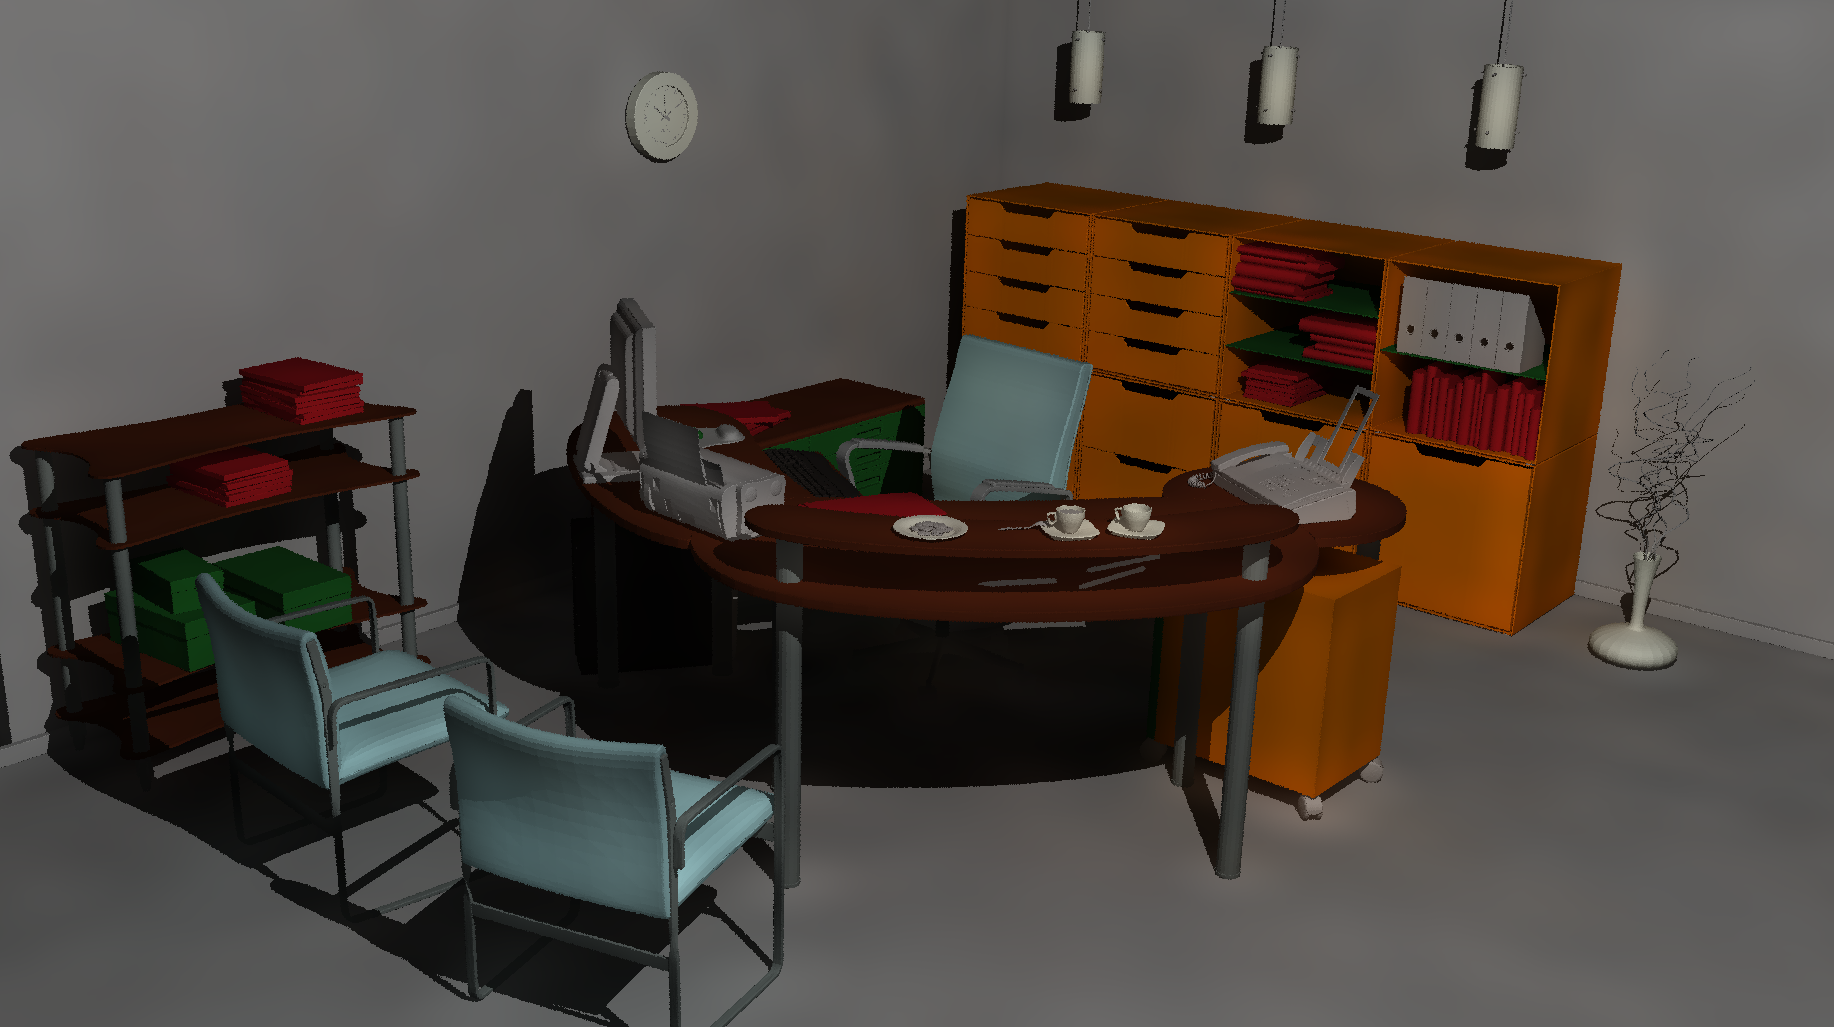
\includegraphics[width=16cm]{pic/office.png}
            \caption{Office最终渲染效果}
            \label{fig:10}
        \end{figure}

        此外,我们还发现光子映射对于画质的真实感有较大提升。如下图所示,从左至右依次为全局光照,直接光照和间接光照图,从上至下依次为
        办公室整体场景、蓝色椅子背部、键盘架附近和办公椅下方:
        \begin{figure}[H]
            \centering
            \subfigure{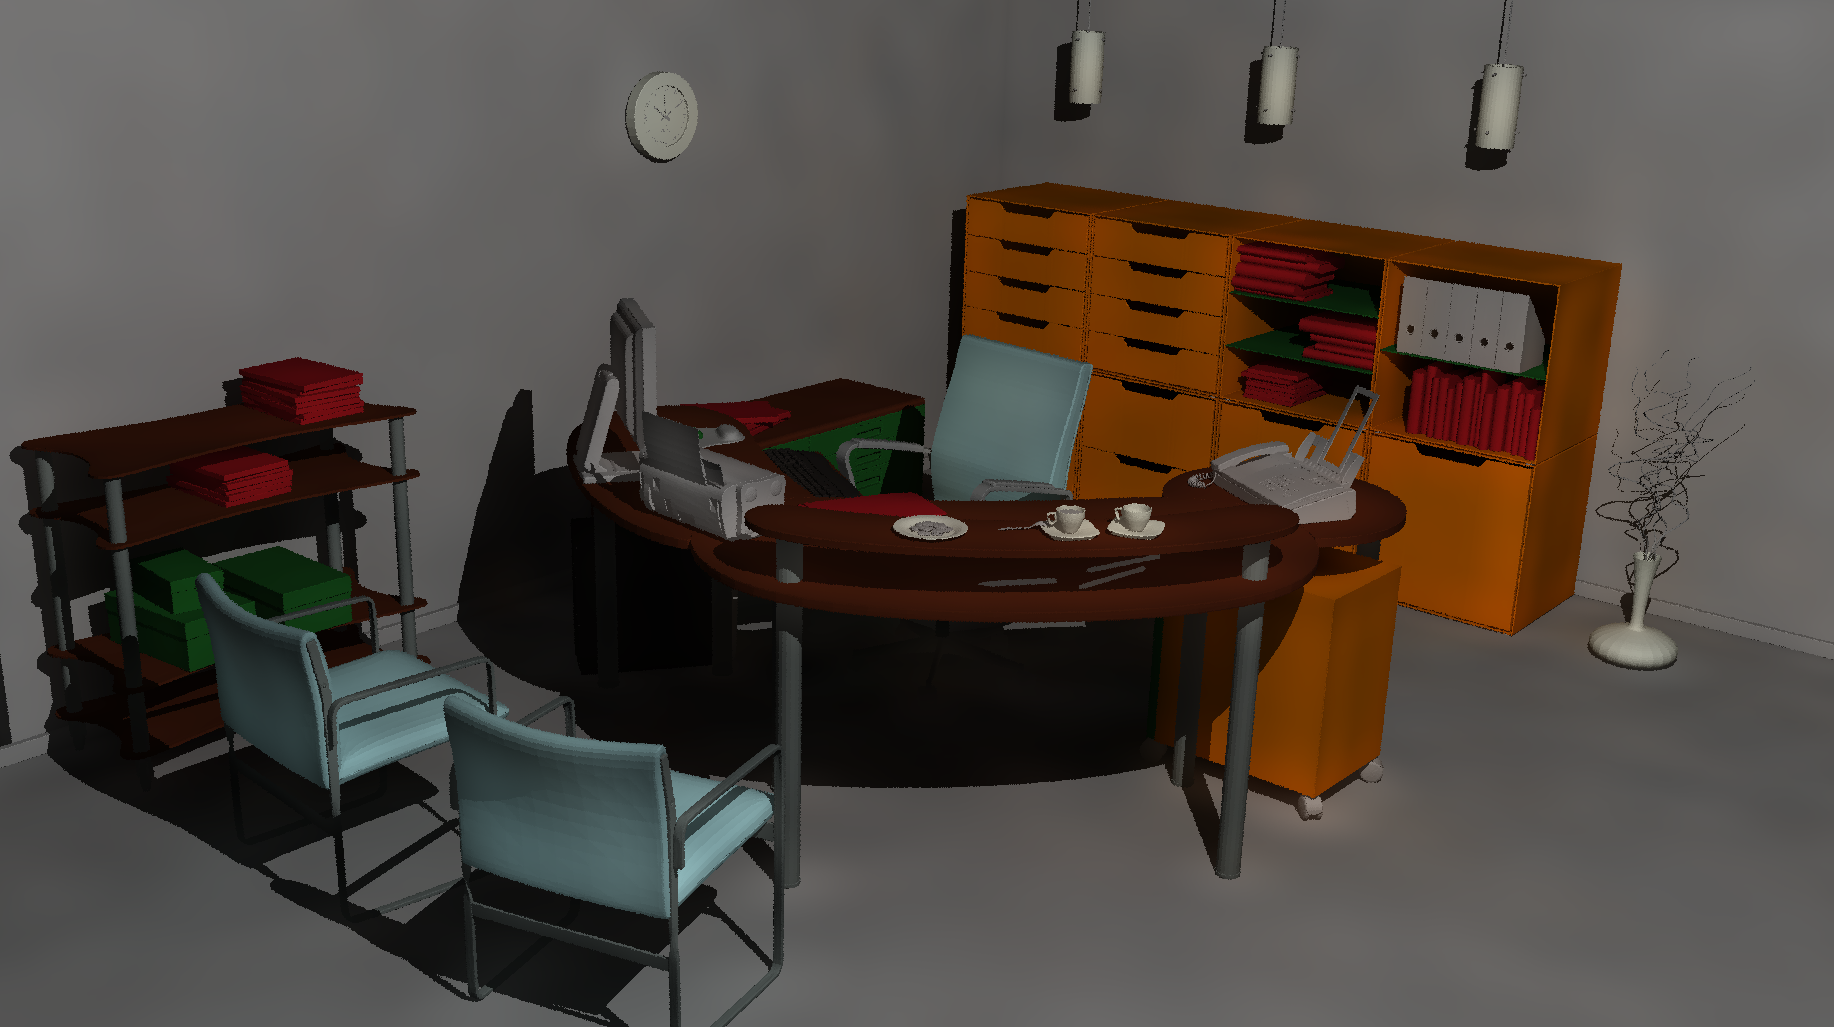
\includegraphics[width=5.5cm]{pic/office.png}}
            \subfigure{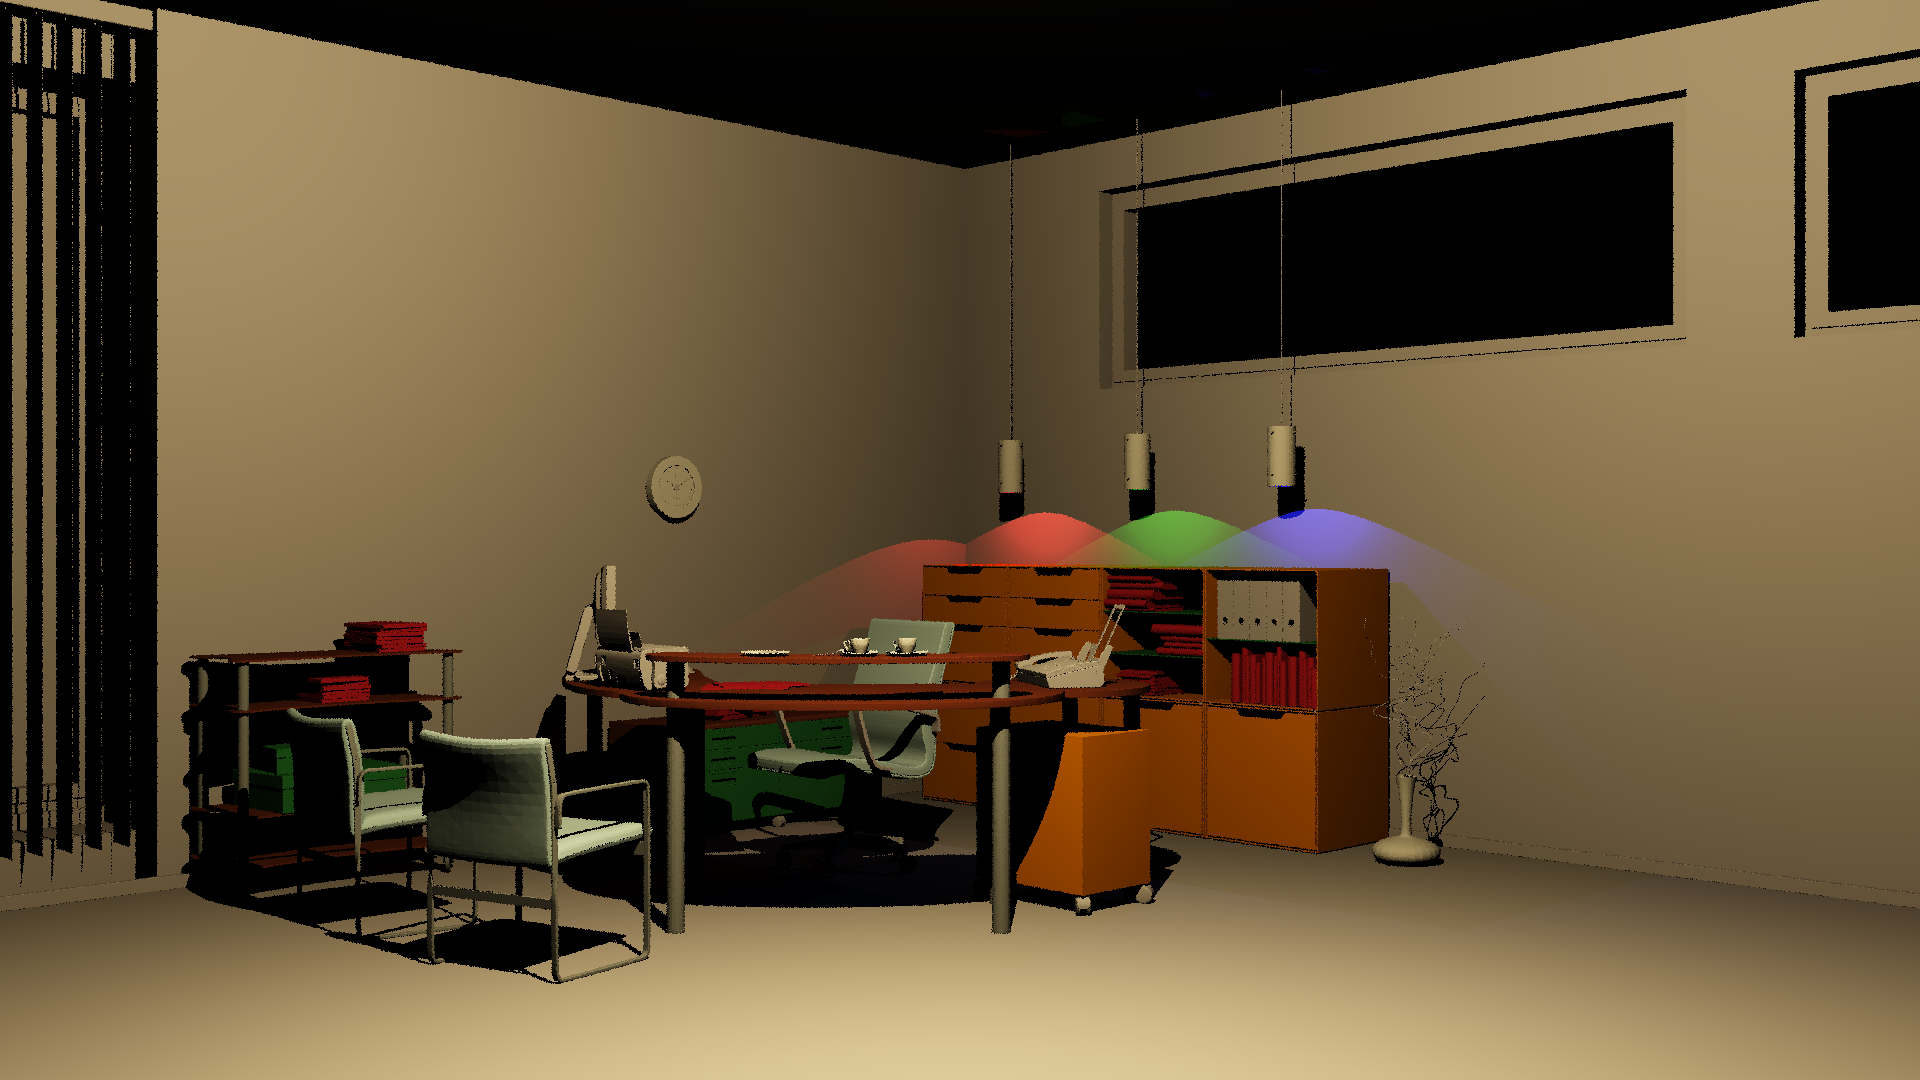
\includegraphics[width=5.5cm]{pic/office_direct.png}}
            \subfigure{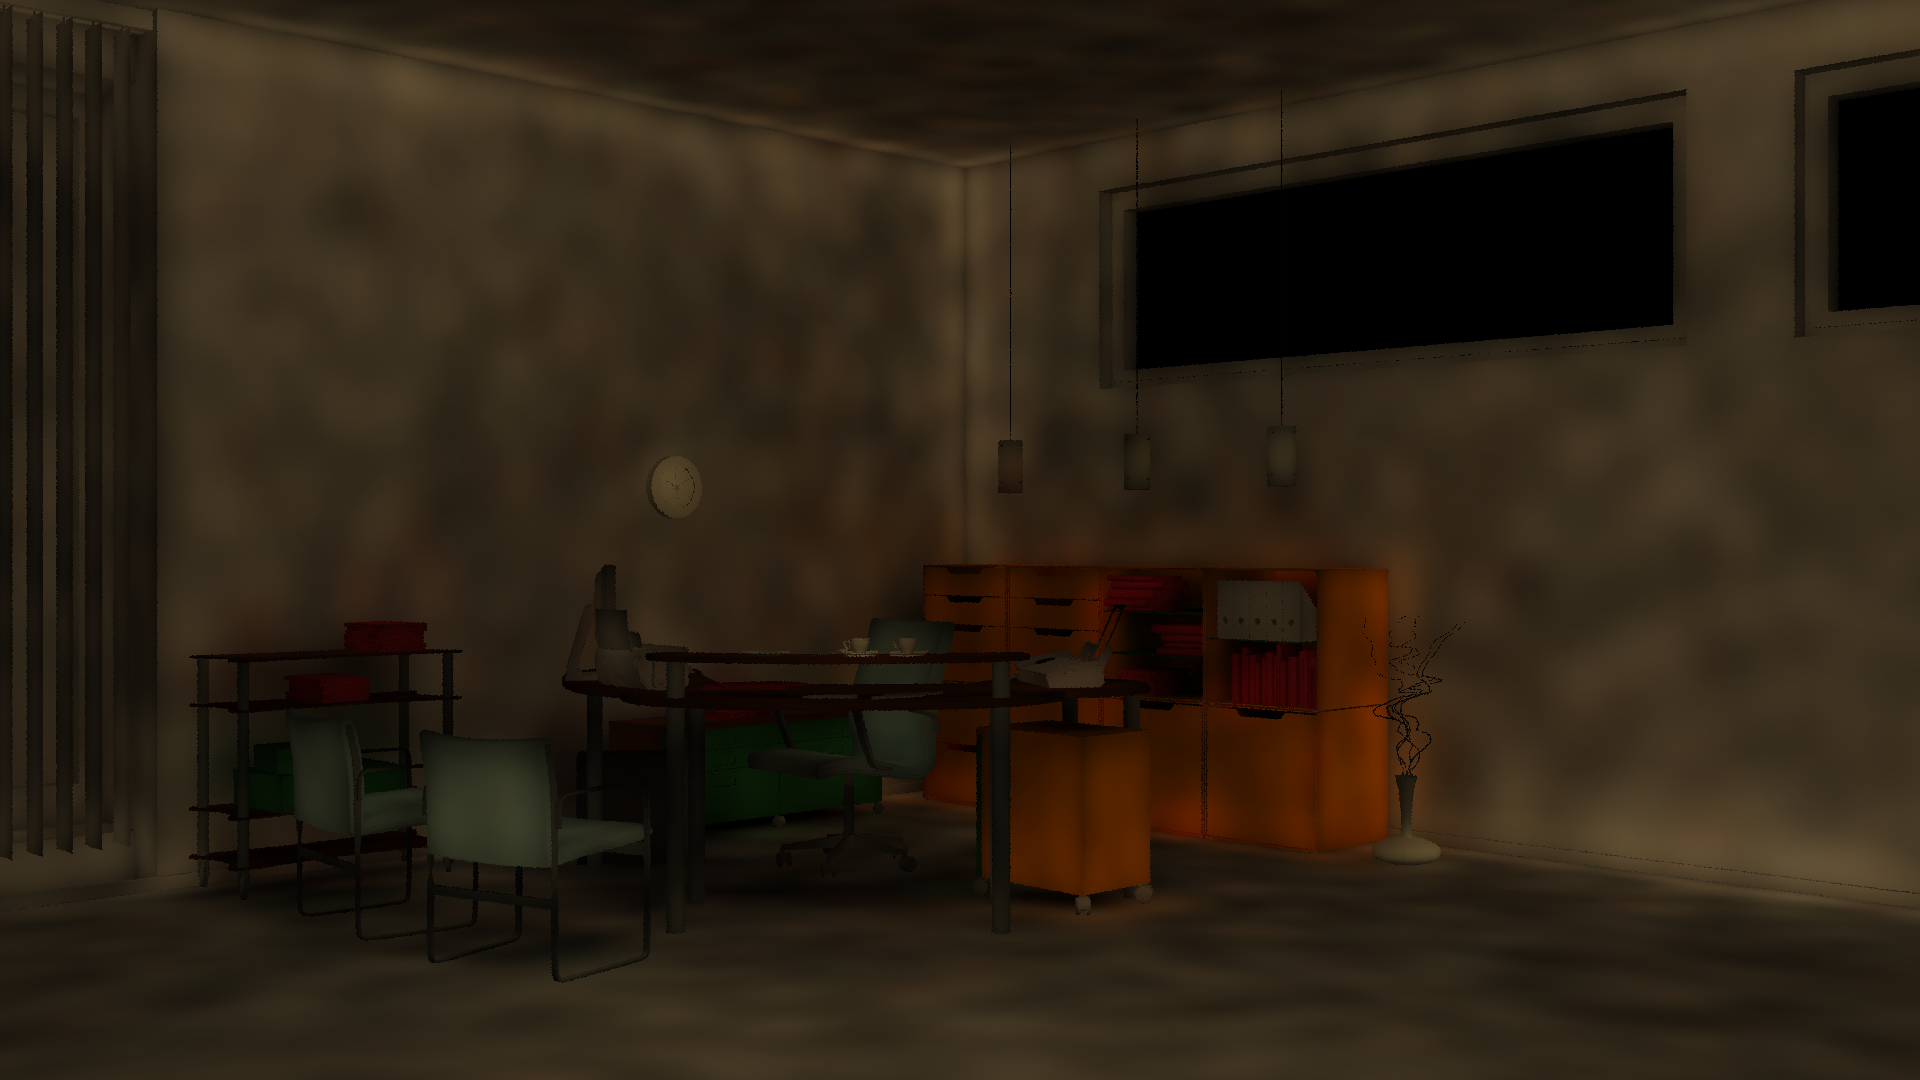
\includegraphics[width=5.5cm]{pic/office_indirect.png}}
            \subfigure{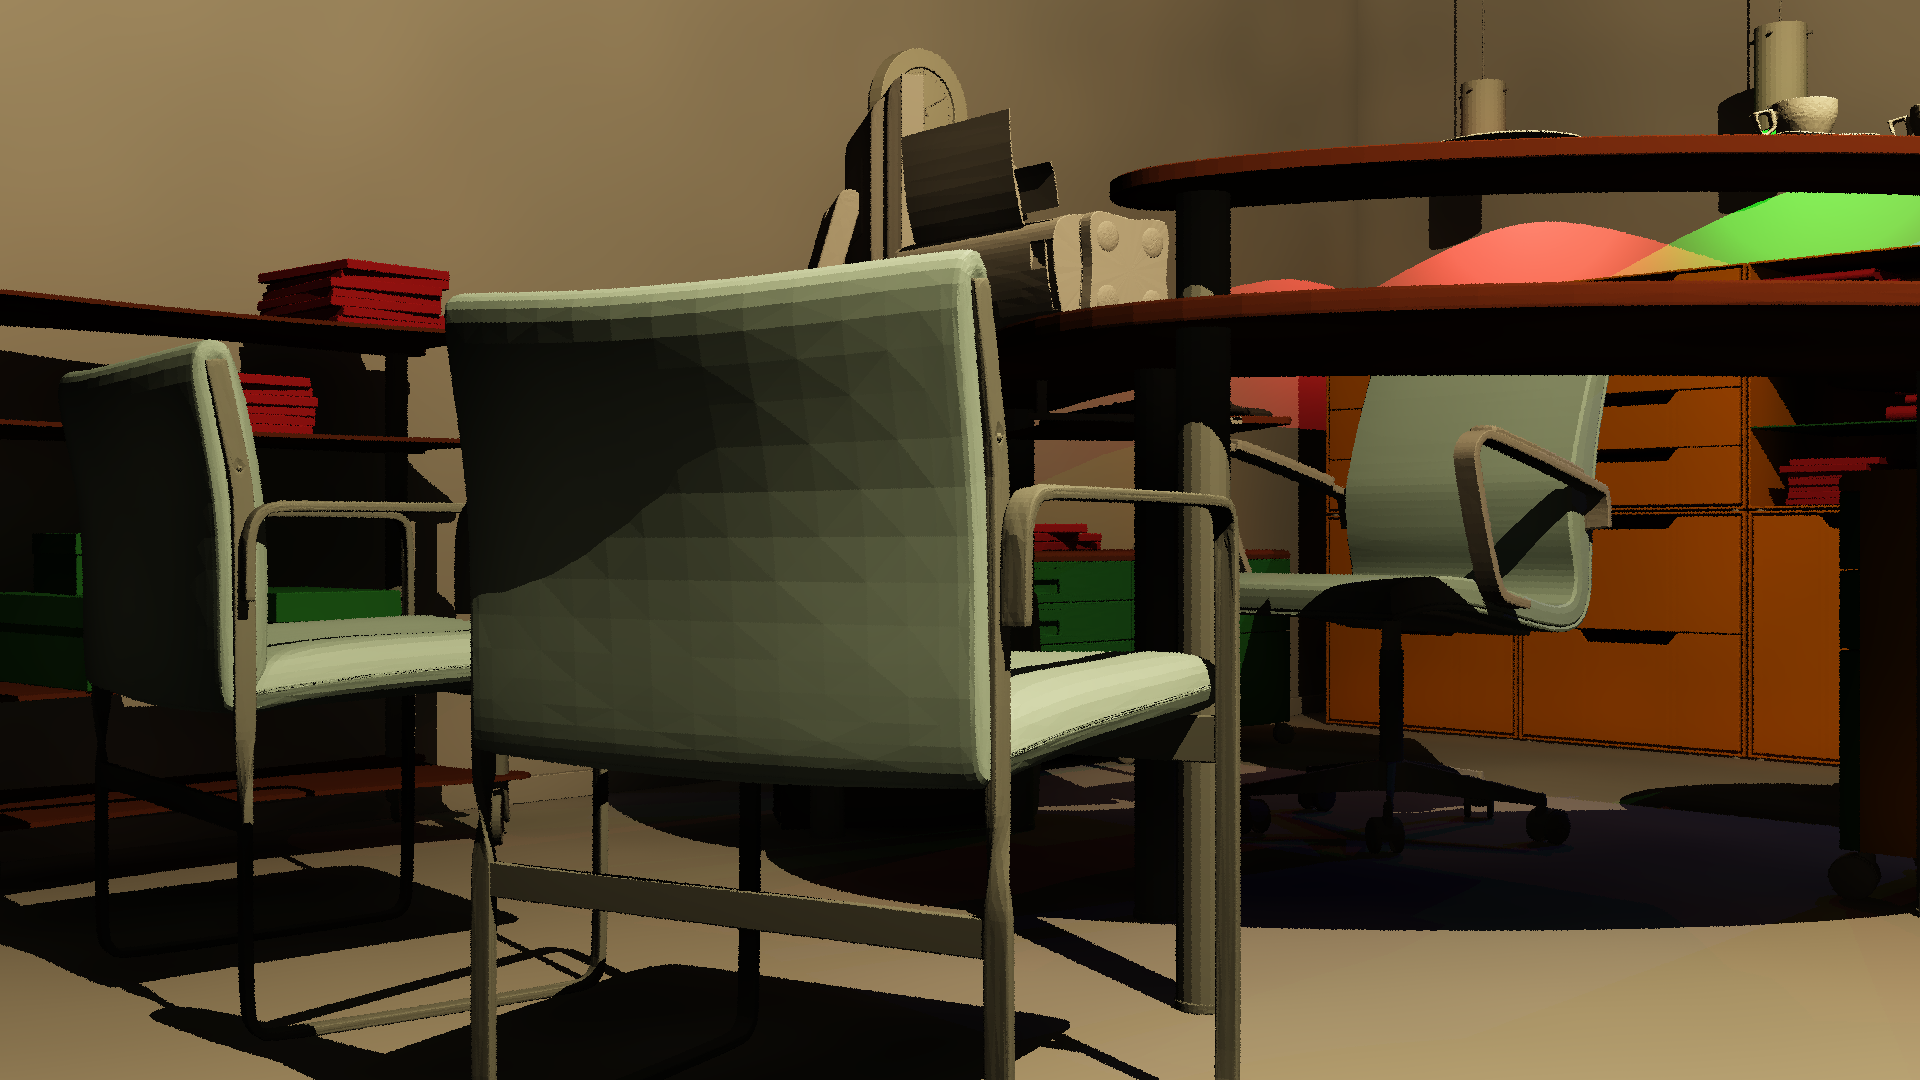
\includegraphics[width=5.5cm]{pic/chair.png}}
            \subfigure{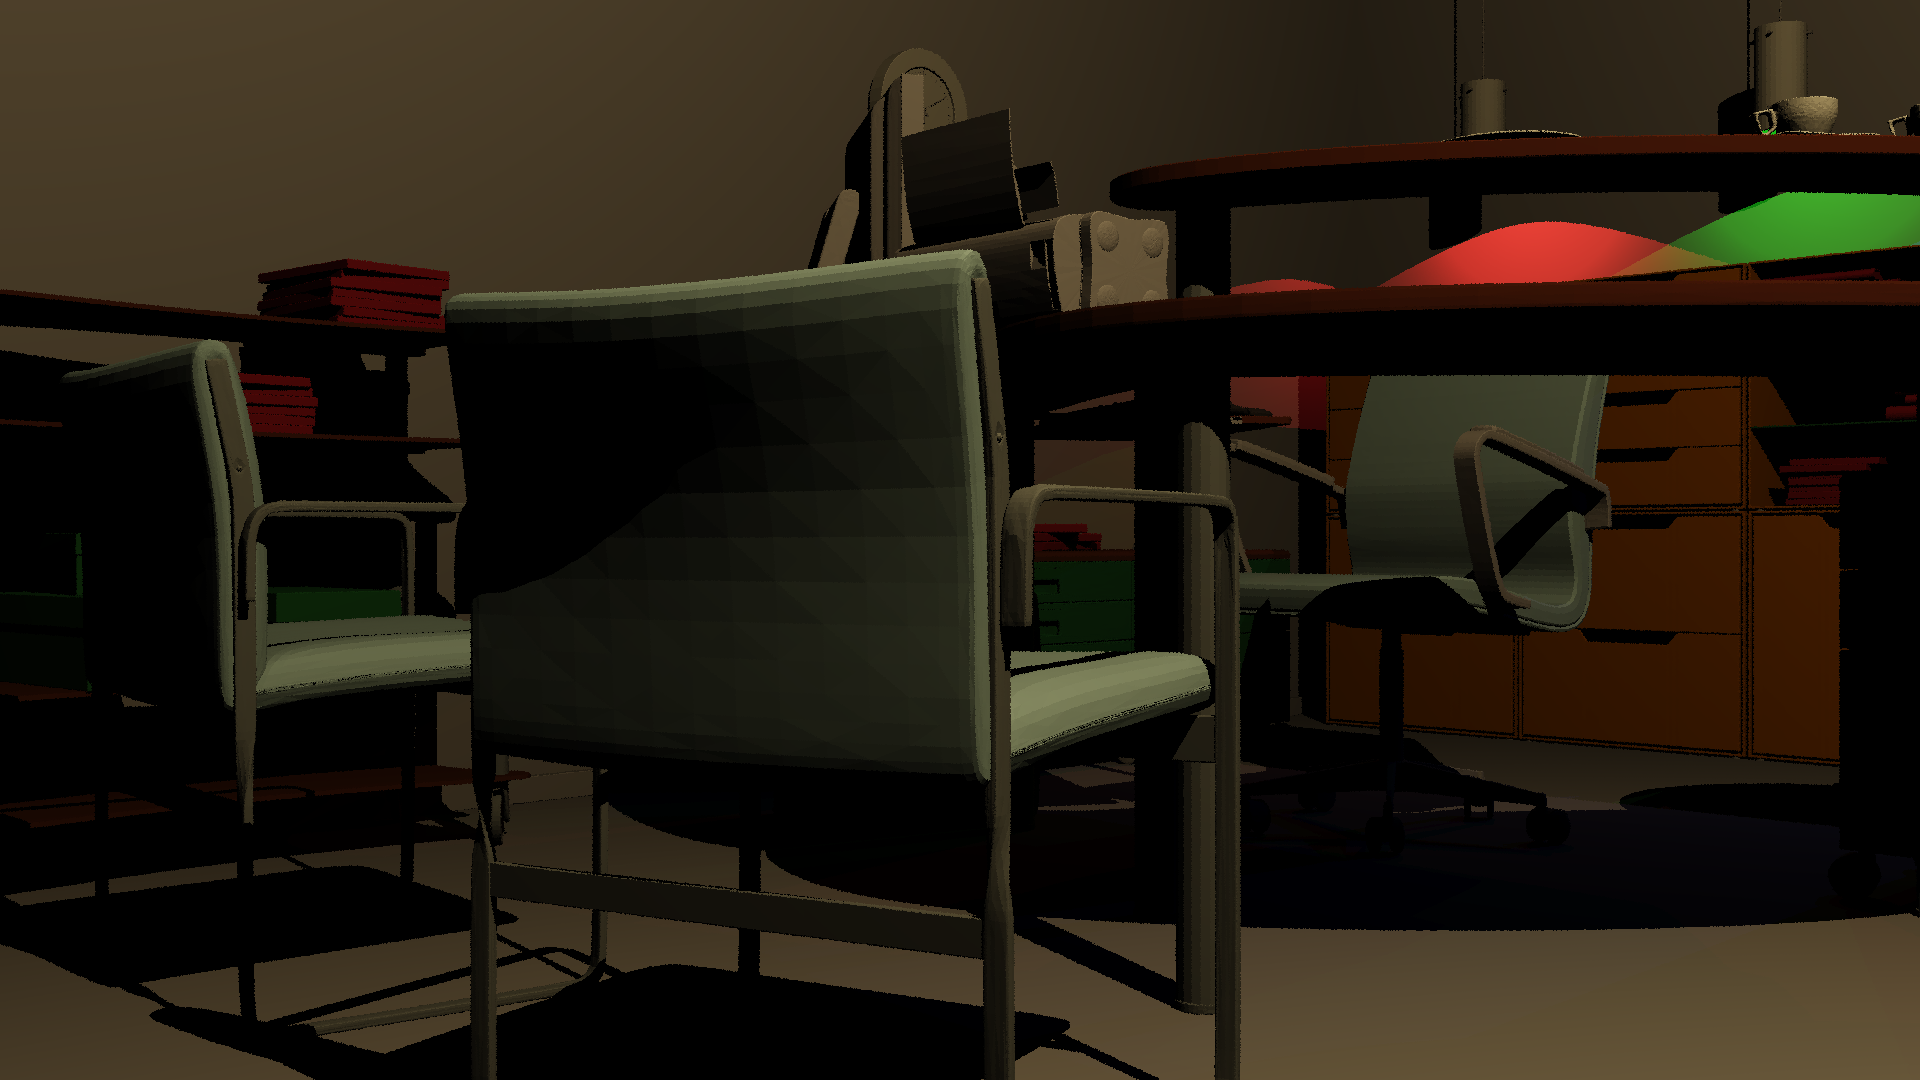
\includegraphics[width=5.5cm]{pic/chair_direct.png}}
            \subfigure{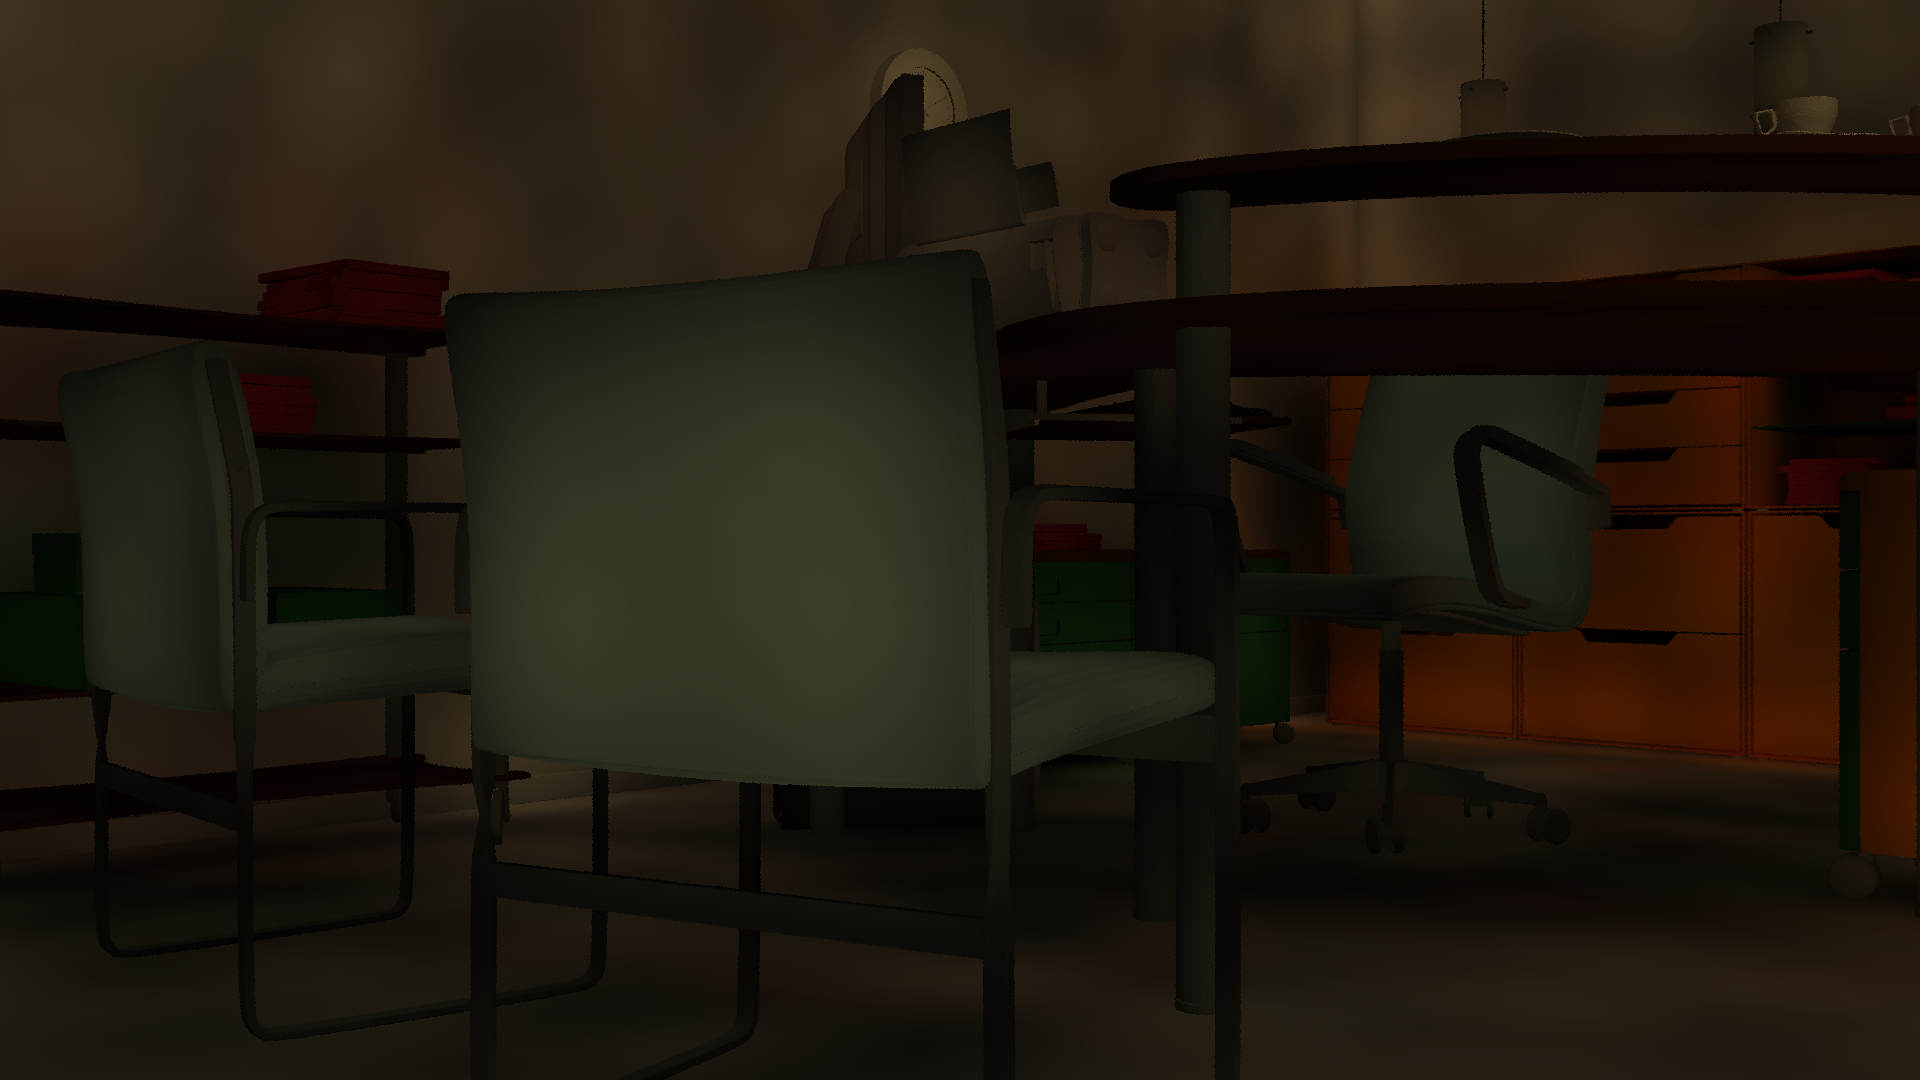
\includegraphics[width=5.5cm]{pic/chair_indirect.png}}
            \subfigure{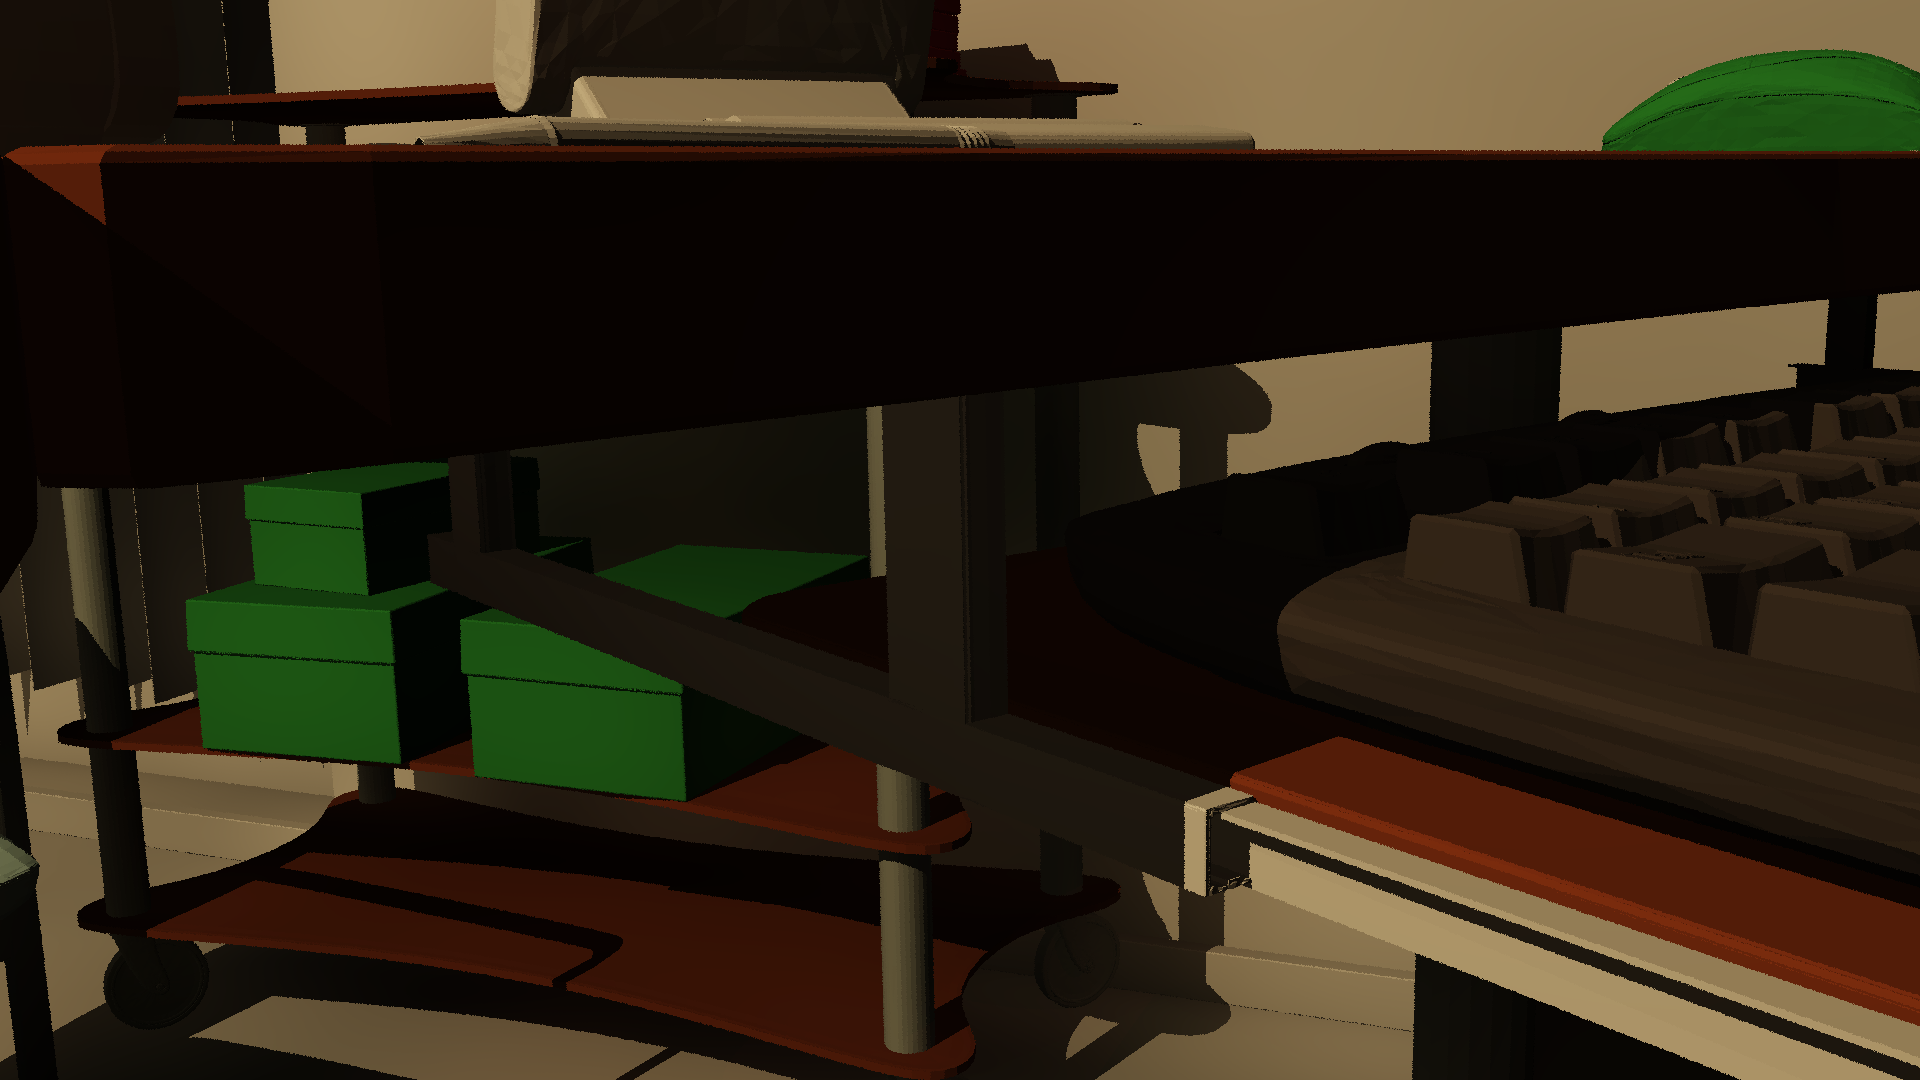
\includegraphics[width=5.5cm]{pic/keyboard.png}}
            \subfigure{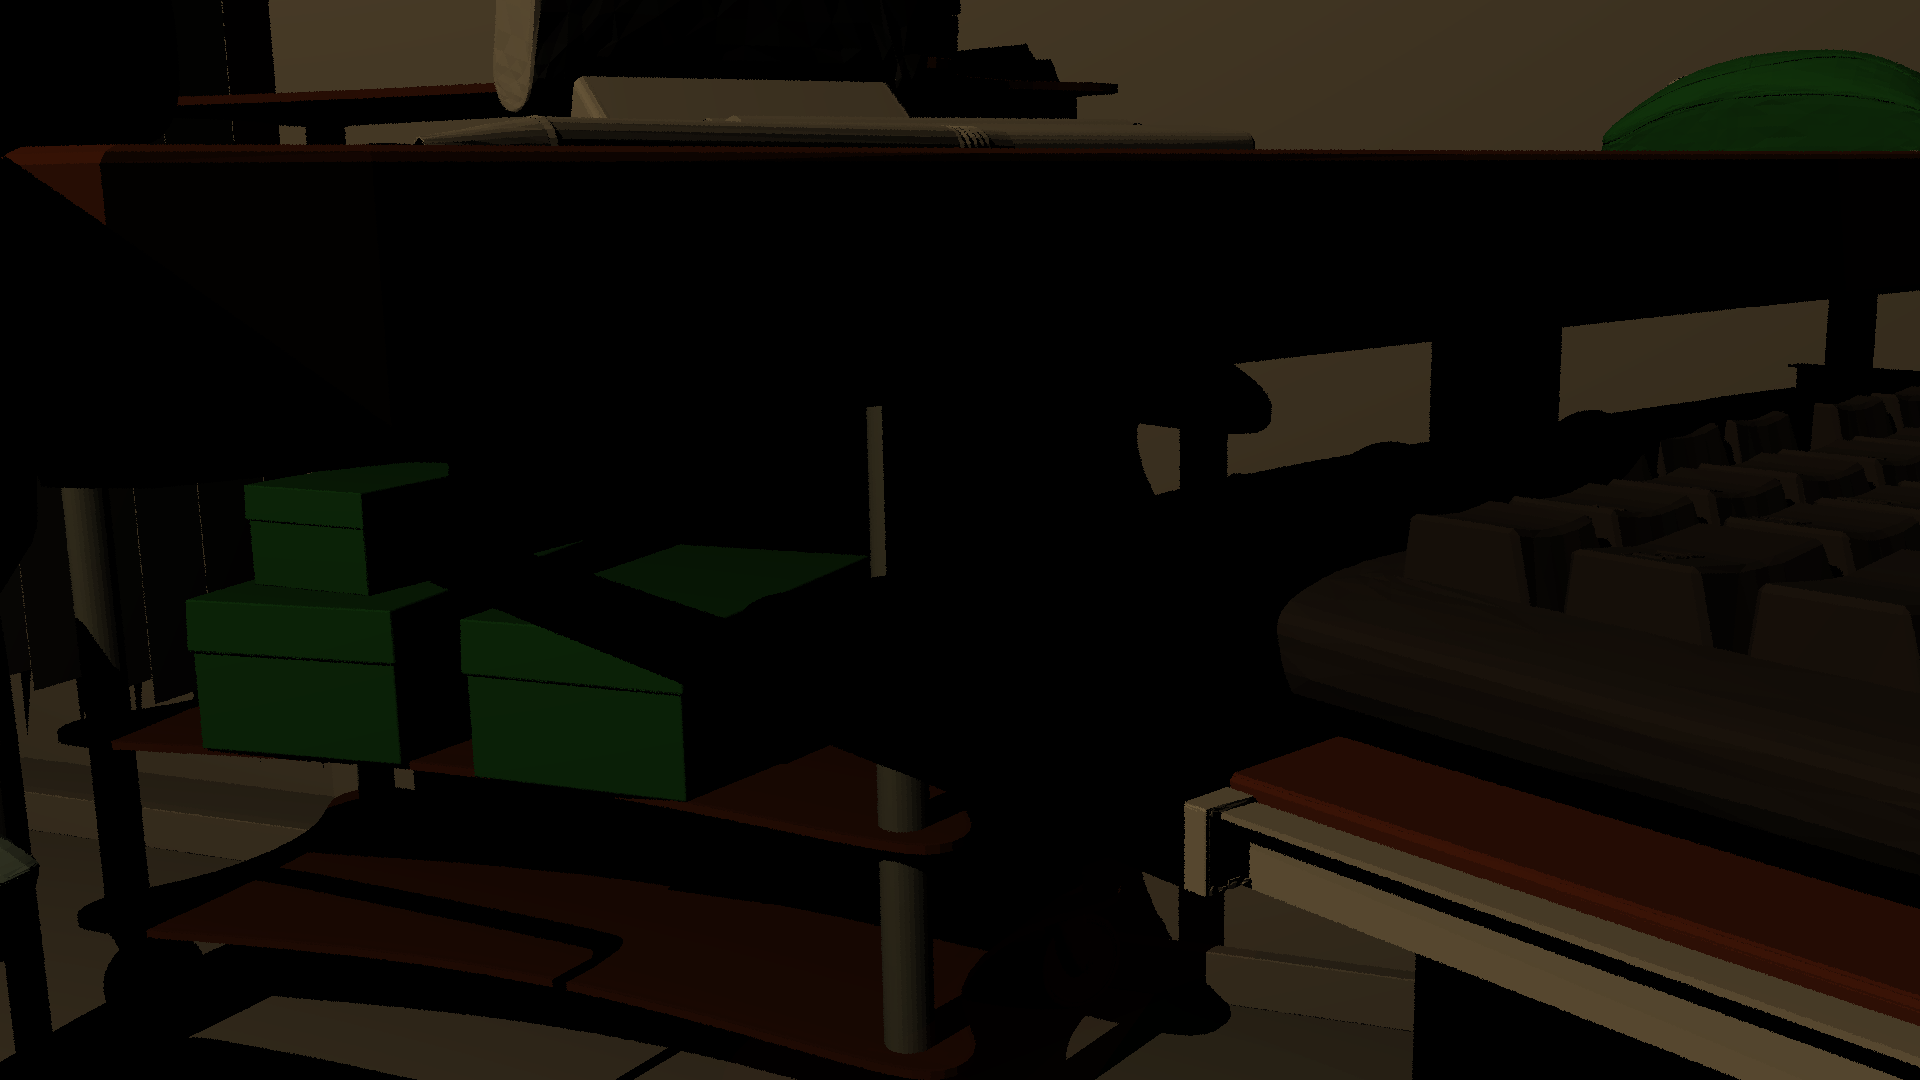
\includegraphics[width=5.5cm]{pic/keyboard_direct.png}}
            \subfigure{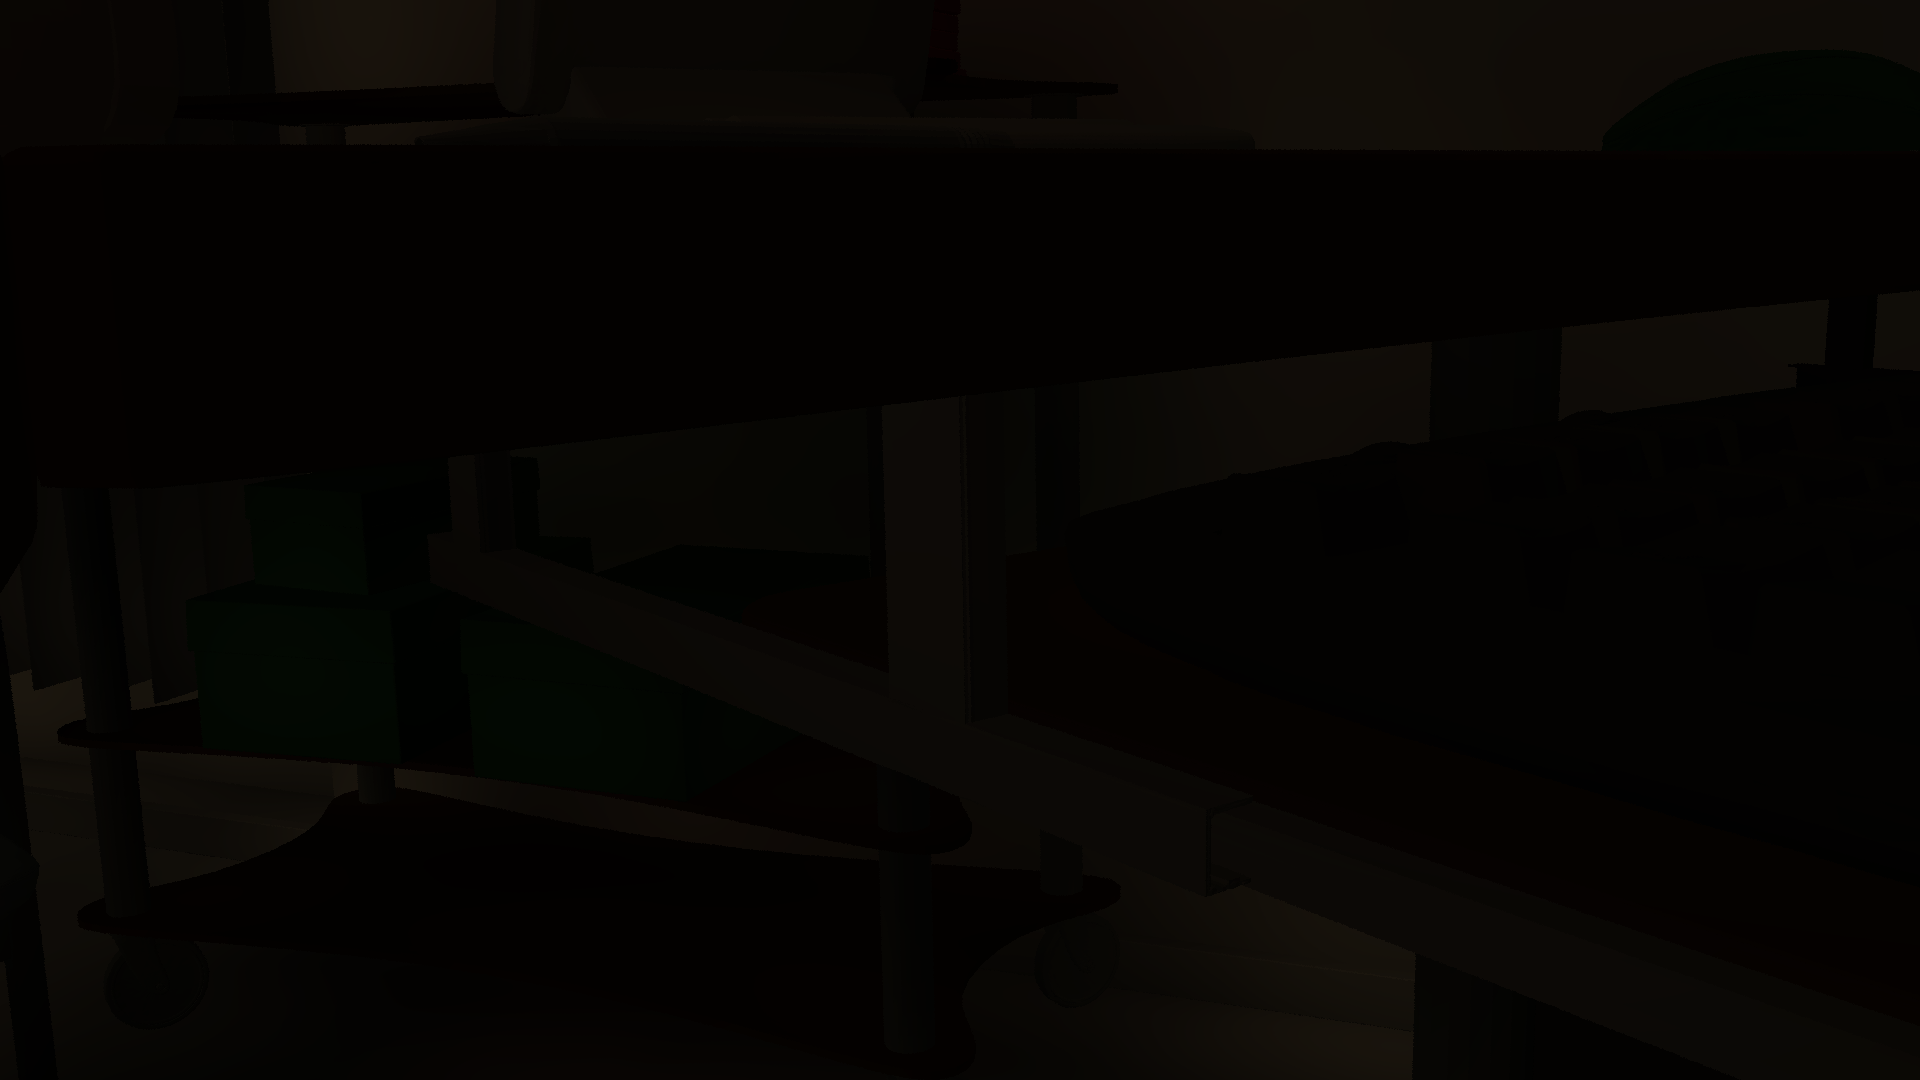
\includegraphics[width=5.5cm]{pic/keyboard_indirect.png}}
            \subfigure{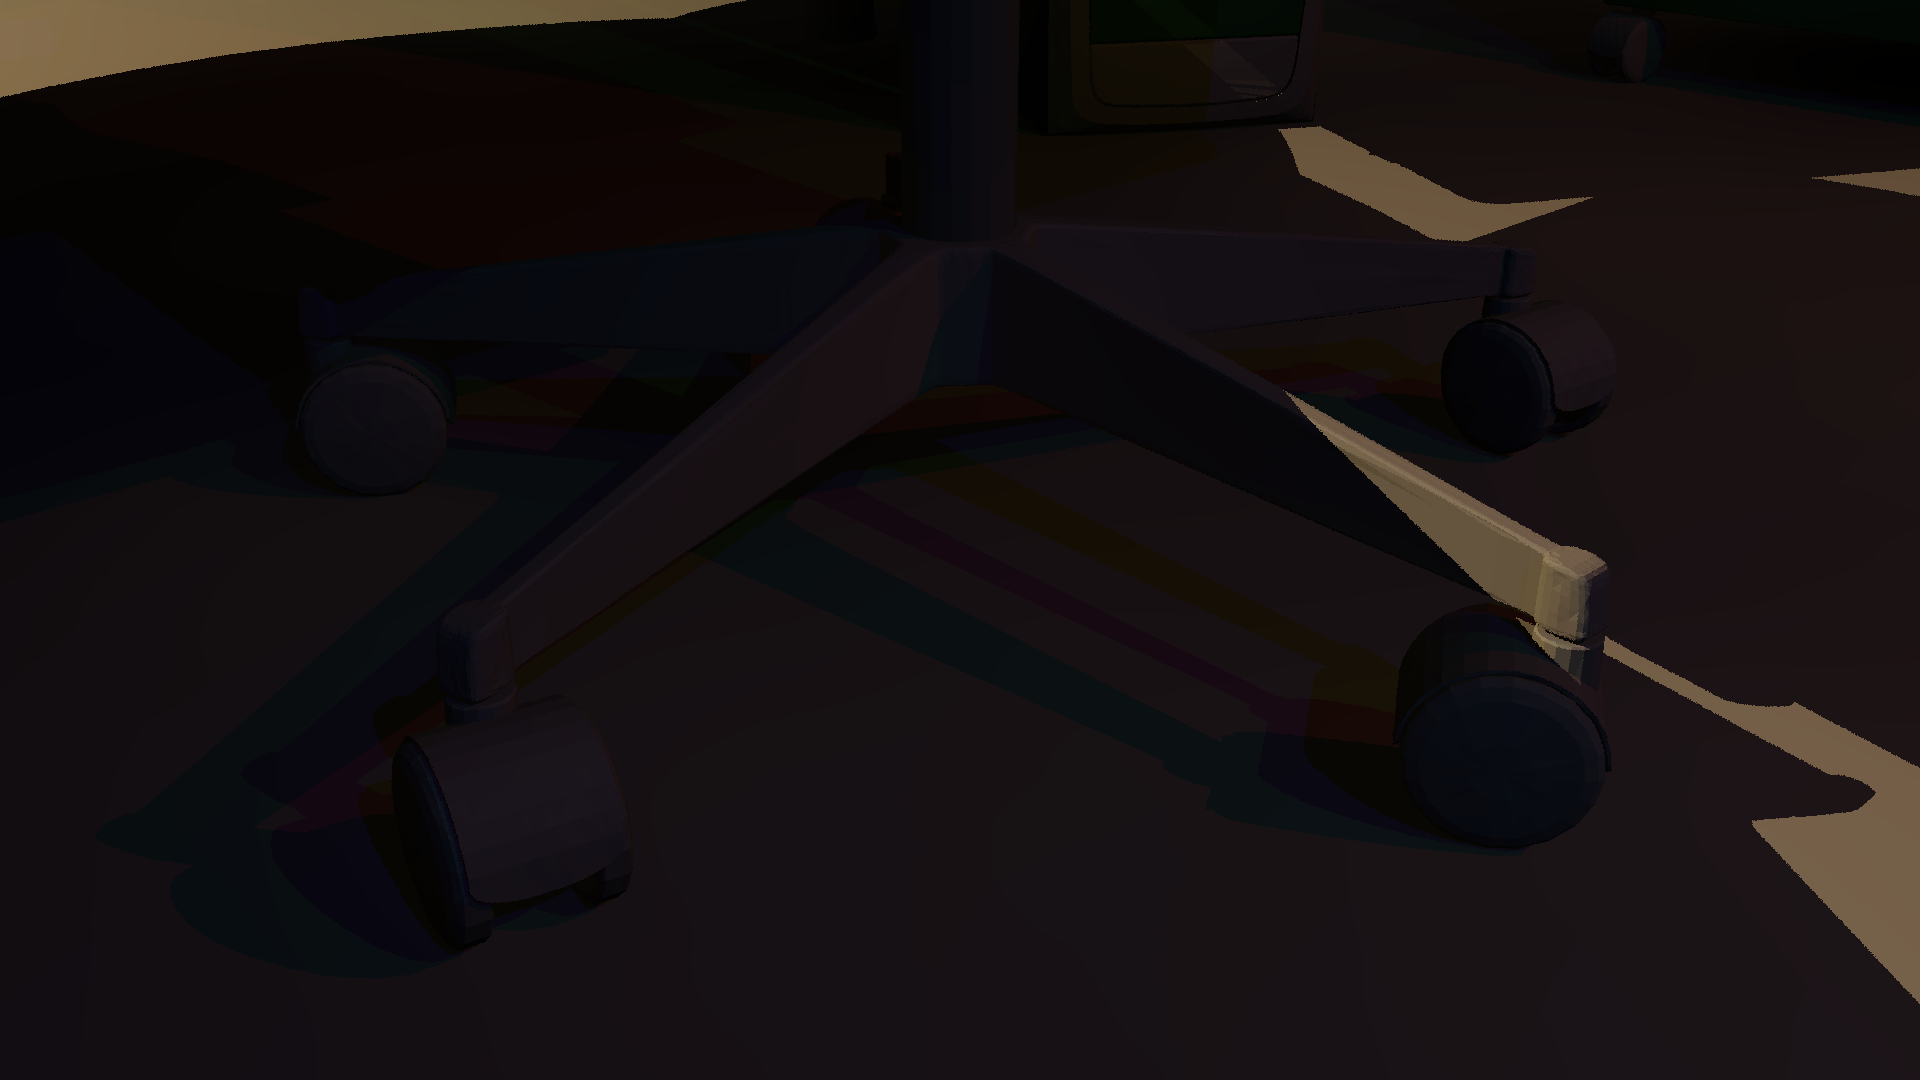
\includegraphics[width=5.5cm]{pic/under_chair.png}}
            \subfigure{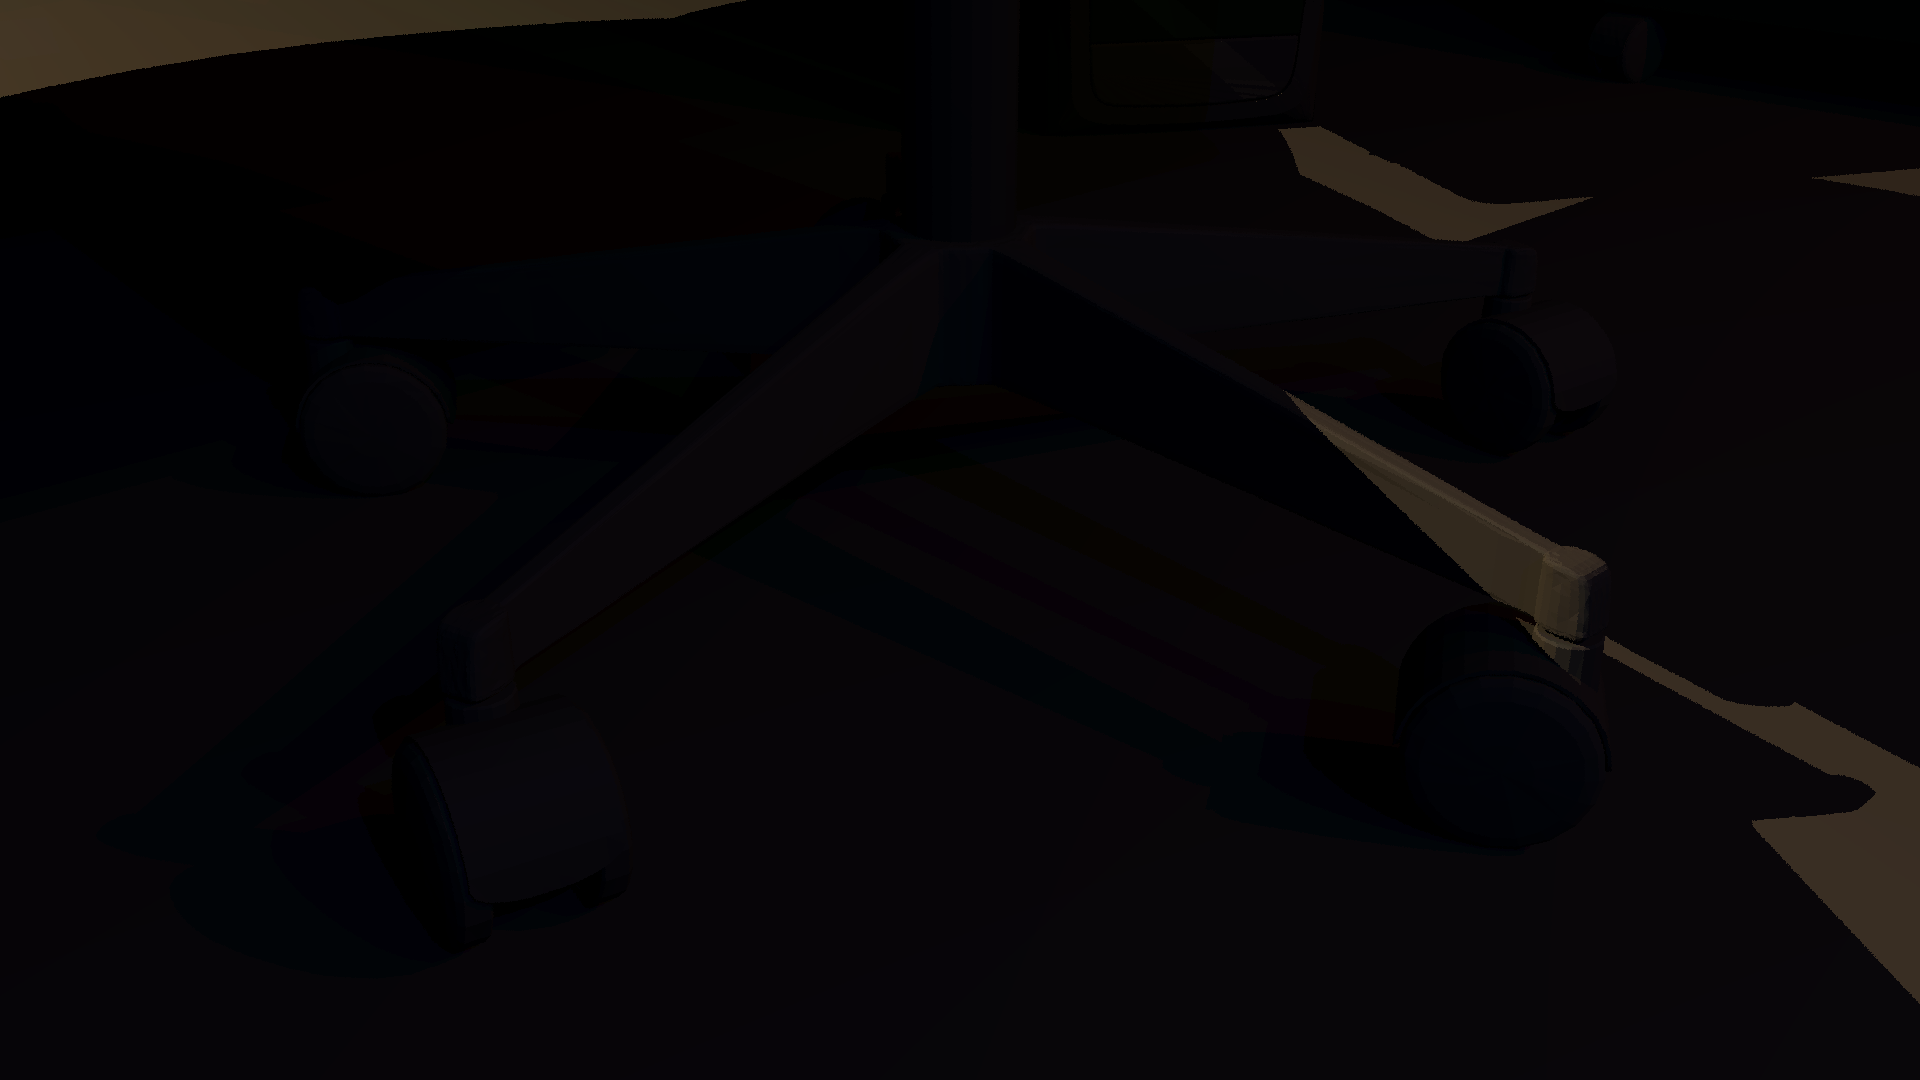
\includegraphics[width=5.5cm]{pic/under_chair_direct.png}}
            \subfigure{
\includegraphics[width=5.5cm]{pic/under_chair_indirect.png}}
        \end{figure}
        在蓝色椅子背部可以看到,光子映射显著增强了亮处和暗处的亮度,还有键盘附近可以发现光子映射让本来完全处于阴影区的键盘支架导轨
        变得可见,使办公椅下面的RGB灯光产生的光照产生的阴影更加真实。

\section{结论}
    基于OptiX光线追踪引擎,我们搭建了一个VR平台上高度真实感绘制的框架,为VR设备上的真实感渲染提供了平台。通过实验验证,我们证明了利用VR设备
    双眼图像之间的相关性避免重复的操作,以加速绘制的过程是可行的。通过改善内存访问模式和充分利用硬件设备进行并行计算,我们对基于光子映射的渲
    染过程进行了加速,最终满足了实时渲染所需要的帧率要求。

\section{不足和改进}
    我们提出了一种在哈希网格结构下利用GPU的共享内存来加速进行密度估计的方案,尽管这一方法并没有带来明显的加速,但是仍有很大的改进空间,比如可以放宽
    启用共享内存的限制条件,充分利用带宽的效率。在\cite{gross2019fast}中提出了一种基于GPU共享内存的近邻搜索方法,或许可以为未来的改进提供思路。

    在我们的实现中,所有点的密度估计都是采用公式\ref{equ:1}进行估计,与给定点不在同一个平面上的光子将被舍去,这样的话在物体边缘的区域,所使用的估计半径
    就会偏大,导致亮度偏低,这一现象称为“边缘偏差”。在\cite{biasControl}中提出了控制偏差的方法,可以为改善渲染效果提供思路。

    此外,人眼具有如下的特性:即对视野中心(也称为注视点\cite{Guenter2012Foveated})最敏感。利用这一特性,可以依据像素位置来调整渲染的精细度,使得中心区域的采样素密度达到最高,
    而周围区域采样密度逐渐递减。通常这块区域是对双眼同时可见的,也就是说对于同一个采样点只需要进行一次光子的收集,这样可以在不影响观感的前提下进一步提升渲染效率。
\bibliography{ref}

\end{document}
